\documentclass[11pt]{article}
\usepackage[margin=1in]{geometry}
\usepackage{amsmath,amssymb,amsthm}
\newtheorem{definition}{Definition}
\usepackage{booktabs}
\usepackage{graphicx}
\usepackage{array}
\usepackage{xcolor}
\usepackage{algorithm}
\usepackage{algpseudocode}
\usepackage{hyperref}
\usepackage{enumitem}
\usepackage{tikz}
\usepackage{pgfplots}
\pgfplotsset{compat=1.17}
\usetikzlibrary{arrows.meta,positioning,shapes.geometric,fit}
\usepackage{subcaption}
\usepackage{rotating} % sidewaystable for the master classification table

% --- notation macros (carried from Paper A v1 for consistency) ---
\newcommand{\R}{\mathbb{R}}
\newcommand{\Q}{\mathbf{Q}}
\newcommand{\X}{\mathbf{X}}
\newcommand{\uu}{\mathbf{u}}
\newcommand{\yy}{\mathbf{y}}
\newcommand{\Amat}{\mathbf{A}}
\newcommand{\W}{\mathbf{W}}
\newcommand{\Imat}{\mathbf{I}}
\newcommand{\bphi}{\boldsymbol{\phi}}
\newcommand{\bmu}{\boldsymbol{\mu}}
\newcommand{\bSigma}{\boldsymbol{\Sigma}}
\newcommand{\bLambda}{\boldsymbol{\Lambda}}

% --- visible TODO macro (results/implementation not yet landed) ---
\newcommand{\TODO}[1]{{\color{red}\textbf{[TODO:} \textsf{#1}\textbf{]}}}
% cmark/xmark/pmark for the capability tables
\newcommand{\cmark}{\ding{51}}
\newcommand{\xmark}{\ding{55}}
\usepackage{pifont}
\newcommand{\pmark}{$\sim$}

\title{\textbf{The Interview-Compatible Recommender:\\A Measuring Instrument for Cold-Start Conversational Recommendation}\\[4pt]\large Thesis Chapter A (v2)}
\author{}
\date{July 2026}

\begin{document}
\maketitle

\begin{abstract}
\noindent Before one can study \emph{how} to interview a cold-start user---which questions to ask, in what
order---one needs a recommender that can \emph{be} interviewed: a model that folds an arbitrary-length,
mixed-channel set of answers into its belief and re-ranks a large catalogue, without per-user retraining and
without trading away full-profile accuracy. We argue that this recommender is a \emph{measuring instrument} for the
entire elicitation-policy literature, and that its requirements are more demanding than any single published system
meets. We state five requirements---\textbf{R1} state-of-the-art full-profile accuracy, \textbf{R2} arbitrary-length
cold-start fold-in, \textbf{R3} channel-agnostic input (items, out-of-catalogue concepts, entities, and continuous
directions through one interface), \textbf{R4} an uncertainty-native belief, and \textbf{R5} monotonicity (a
truthful answer never lowers ranking quality)---and an acceptance battery (per-build gates \textbf{G0--G9} plus
one-time certifications \textbf{C1--C3}) that operationalises them. A survey of six model families shows the literature is \emph{bifurcated}: the models that hit
the full-profile bar (shallow linear/autoencoder recommenders such as EASE~\cite{steck2019ease} and
RecVAE~\cite{ren2020recvae}) are item-only point estimators, while the models with an uncertainty-native, multi-channel
belief (soft-attribute Gaussian elicitation~\cite{biyik2023soft}, unified item$+$attribute bandits~\cite{li2021seamlessly},
conjugate critique folds~\cite{toroghi2023bcie}) do not report full-profile accuracy at the R1 bar. We are aware of no
published system that occupies the conjunction of all five. The instrument we propose to close this gap is a
\emph{frozen} certified shallow-SOTA tower with an analytic conjugate-Gaussian belief layer over its latent, into
which every channel folds as a linear observation; three of its input legs---signed/graded values, out-of-catalogue
concepts, and continuous direction tokens---are architecturally inexpressible in the item-indicator basis of the R1-bar
models. This chapter contributes the requirement framework, the taxonomy and gap analysis, the instrument's design,
and the experimental protocol (a metric-certification bridge to the published ML-20M numbers, then G0/G1/G2 on the
ML-25M harness). Our in-house RecVAE realisation sets the current bar at full/tail NDCG@10 $0.3540/0.2497$ on the
canonical ML-25M protocol; the graded-native interview tower is training and all instrument results are marked
\TODO{} pending certification.
\end{abstract}

\tableofcontents

% =====================================================================
\section{Introduction: the recommender as a measuring instrument}\label{sec:intro}
% =====================================================================

A \emph{cold-start} conversational recommender must elicit taste from a short interview and then rank a large
catalogue. Two questions are entangled: \emph{what to ask} (the elicitation policy) and \emph{how to turn answers
into recommendations} (the recommender). The elicitation-policy literature is large and active, but almost every
comparison in it is confounded: a policy's apparent value depends on the recommender it drives, and reported gains
routinely conflate a better \emph{question-selection strategy} with a better \emph{answer-ingestion model}. Before we
can measure elicitation strategies in isolation, we need to fix the recommender---and not just any recommender, but one
strong and flexible enough that a good interview is not wasted on it. We call such a recommender an
\emph{interview-compatible instrument}.

\paragraph{Five requirements.}
An instrument fit for measuring conversational elicitation must simultaneously satisfy:
\begin{description}[leftmargin=2.4em,itemsep=1.5pt]
  \item[R1 --- full-profile SOTA.] On a full interaction history it must rank at the level of the strongest shallow
        collaborative-filtering baselines (EASE~\cite{steck2019ease}, RecVAE~\cite{ren2020recvae}), so that
        elicitation is measured against a recommender nobody can dismiss as weak~\cite{dacrema2019progress}.
  \item[R2 --- any-length cold-start fold-in.] It must ingest an evidence set of \emph{any} cardinality, from $0$
        (fully cold) upward, without per-user retraining.
  \item[R3 --- channel-agnostic input.] Items, out-of-catalogue concepts, entities, and free text (and, for the
        continuous policy, direction tokens) must all fold through \emph{one} interface as arbitrary embeddings, not a
        fixed categorical schema.
  \item[R4 --- uncertainty-native belief.] It must carry an explicit covariance over the user belief, not just a
        point estimate, so that a policy can act on \emph{what it does not yet know}.
  \item[R5 --- monotonicity.] A truthful answer must never \emph{lower} ranking quality; adding evidence should, in
        expectation, only help.
\end{description}

\paragraph{The bifurcation observation.}
The central empirical fact this chapter documents is that R1 and $\{$R3, R4, R5$\}$ are \emph{anti-correlated across
the published literature}. The models that hit the full-profile bar---closed-form linear autoencoders
(EASE~\cite{steck2019ease}, EDLAE~\cite{steck2020edlae}), amortised VAEs (Mult-VAE~\cite{liang2018variational},
RecVAE~\cite{ren2020recvae}), and training-free graph filters
(GF-CF~\cite{shen2021gfcf}, BSPM~\cite{choi2023bspm}, Turbo-CF~\cite{park2024turbocf})---are \emph{item-only point
estimators} on a one-hot indicator basis. The models with an uncertainty-native, multi-channel belief---soft-attribute
Gaussian elicitation~\cite{biyik2023soft}, item$+$attribute Thompson bandits~\cite{li2021seamlessly}, conjugate critique
folds over a frozen factorisation~\cite{toroghi2023bcie}, and per-item Bayesian NL elicitation~\cite{austin2024bayesian}---do
\emph{not} report full-profile accuracy at the R1 bar. We call these the \emph{accuracy corner} and the \emph{belief
corner}. No published system we are aware of occupies both (\S\ref{sec:gap}).

\paragraph{Contributions.}
This chapter is the instrument paper of the thesis. It does not claim a new elicitation policy (that is the companion
method chapter); it claims the \emph{recommender that makes policy measurement possible}. Concretely:
\begin{enumerate}[leftmargin=1.5em,itemsep=1.5pt]
  \item \textbf{The conjunction as the contribution.} We frame R1$\wedge$R2$\wedge$R3$\wedge$R4$\wedge$R5 as a single
        requirement no published system meets, and give a six-family taxonomy and per-near-miss gap analysis
        (\S\ref{sec:related},~\S\ref{sec:gap}) that locates exactly which requirement each candidate fails. We say we
        are \emph{aware of none}, never that there \emph{is} none.
  \item \textbf{Three architecturally-inexpressible legs.} We isolate the three input channels that are impossible
        (not merely untuned) in the item-indicator basis of every R1-bar model: (i) signed/graded per-entity values,
        (ii) out-of-catalogue concepts, and (iii) continuous direction tokens. These are the narrow, defensible novelty
        legs of the channel-agnostic interface (\S\ref{sec:gap},~\S\ref{sec:method}).
  \item \textbf{The instrument.} A design for a \emph{frozen} certified shallow-SOTA tower with an analytic
        conjugate-Gaussian precision-accumulator belief layer over its latent, into which every channel folds as a
        linear observation (\S\ref{sec:method}). The frozen-tower$+$exact-conjugacy shape is the one mechanism with a
        principled monotonicity story~\cite{toroghi2023bcie}, and it is what separates us from the co-trained,
        approximate-posterior near-miss of Bıyık et al.~\cite{biyik2023soft}.
  \item \textbf{An acceptance battery as a reusable certificate.} We define three headline outcome gates---full-strength
        preserved (G0), posterior strictly shrinks per question (G1), and cold-start per-question NDCG rises on
        \emph{full and tail} versus random (G2)---and, because these outcome gates admit several false positives
        (a sign-blind fold, a circular answer model, a decorative covariance), extend them into a full battery of
        per-build gates G0--G9 plus one-time certifications C1--C3 that add the semantic, artifact-control, and
        answer-model-transfer checks. We propose the battery as a portable certificate any interview-compatible
        recommender should pass (\S\ref{sec:reqs},~\S\ref{sec:expdesign}).
\end{enumerate}

We are careful throughout to distinguish what is \emph{new} (the conjunction; the frozen-certified-tower wedge; the
acceptance battery on a SOTA tower) from what is \emph{pre-empted} and must be cited (attributes-as-directions plus a
Bayesian fold~\cite{biyik2023soft}; unified item$+$attribute belief~\cite{li2021seamlessly}; conjugate folds over a
frozen factorisation~\cite{toroghi2023bcie}; permutation-invariant set-encoders with information-gain
acquisition~\cite{ma2019eddi}; value-carrying set-input cold-start recommenders~\cite{lin2021tanp}; the
non-degradation-of-information principle, Good 1967 / Blackwell). ``Uncertainty-native recommender'' alone is a
crowded 2024--25 area~\cite{wang2025bdecf} and is \emph{not} claimed as novel.

% =====================================================================
\section{Requirements and gates}\label{sec:reqs}
% =====================================================================

We now state the requirements and gates formally. Let the catalogue have $n$ items and let the frozen tower expose a
$d$-dimensional latent in which each item $i$ has a factor row $\Q_i\in\R^{d}$. An \emph{evidence set} after $t$
questions is a set of observations $\mathcal E_t=\{(\bphi_j, y_j)\}_{j=1}^{t}$, where $\bphi_j\in\R^{d}$ is the latent
direction of the queried entity (an item factor, a concept centroid, an entity embedding, or a continuous direction
token) and $y_j\in\R$ is the (possibly graded, possibly signed) answer. The instrument maintains a belief
$b(\mathcal E_t)=(\bmu_t,\bSigma_t)$ over the user latent $\uu\in\R^{d}$ and scores item $i$ by a fixed read-out
$s_i(\bmu_t)$ of the base tower.

\paragraph{Requirements (formal).}
\begin{description}[leftmargin=2.4em,itemsep=1.5pt]
  \item[R1.] With $\mathcal E$ equal to a user's full history, $\mathrm{NDCG}@10\bigl(s(\bmu(\mathcal E))\bigr)$ ties
        the strongest shallow baseline on a shared harness (Def.~\ref{def:tie}).
  \item[R2.] $b(\mathcal E_t)$ is defined and computable for every $t\ge 0$ with no gradient step at inference; $t{=}0$
        yields the prior belief (a non-personalised ranker).
  \item[R3.] The update from $\mathcal E_t$ to $\mathcal E_{t+1}$ depends on the new observation only through the pair
        $(\bphi_{t+1},y_{t+1})\in\R^{d}\times\R$; the operator is identical for every channel, so any entity with an
        embedding is a legal observation---including entities absent from the catalogue.
  \item[R4.] $\bSigma_t$ is an explicit, queryable covariance; a policy may read $\bSigma_t$ to choose the next
        question.
  \item[R5.] For a truthful answer $y_{t+1}$, $\mathbb E\bigl[\mathrm{NDCG}@10(s(\bmu_{t+1}))\bigr]\ge
        \mathrm{NDCG}@10(s(\bmu_t))$. We treat R5 as an \emph{empirical} property to be demonstrated per step, not a
        theorem for a learned ranker (\S\ref{sec:limits}).
\end{description}

\begin{definition}[Ties SOTA]\label{def:tie}
A recommender \emph{ties} a baseline on a metric if their scores are within the paired per-user bootstrap confidence
interval on one shared harness (same users, items, split, metric depth). A number computed on a different
metric/split (e.g.\ NDCG@10 on ML-25M vs.\ NDCG@100 on the ML-20M strong-generalisation split) is \emph{not} a tie
until bridged (\S\ref{sec:bridge}).
\end{definition}

\paragraph{Gates (acceptance battery).}
The three headline gates below (G0/G1/G2) are \emph{outcome} gates: they certify that the full-profile strength is
preserved, that the posterior is usable, and that the cold-start curve rises. On their own they are insufficient
(see below), so the instrument is accepted only against the full battery---per-build gates G0--G9 (every build, all
cheap) and three one-time certifications C1--C3. Table~\ref{tab:battery} is the compact reference; the definitions
follow.

\emph{Per-build gates.}
\begin{description}[leftmargin=2.4em,itemsep=1.5pt]
  \item[G0 --- full strength \& identity.] Evaluating on the belief mean with the full profile reproduces the frozen
        tower's full-profile NDCG@10 (full \emph{and} tail)---a paired-bootstrap tie, or bit-identity under the
        frozen-fold design---so the belief layer adds no full-profile regression (certifies R1 survives).
  \item[G1 --- usable posterior.] The posterior covariance shrinks in expectation over confident answers, with
        \emph{refusals explicitly exempt} (a correct model does not shrink on a refusal); the shrinkage is directional
        (at least twice as large along the queried $\bphi_{t+1}$ as elsewhere) and the belief scale is calibrated
        against held-out NLL (certifies R4).
  \item[G2 --- cold-start curve rises on full and tail.] Starting cold, per-question full and tail NDCG@10 beats a
        random-question control judged by the \emph{curve/endpoint at budget} (an AUC criterion, \emph{not} every-step
        significance), and must strictly \emph{increase} from the first to the last turn (not merely fail to drop);
        plus an out-of-envelope canary that a single true answer from cold helps on \emph{every} channel. This is the
        operational form of R2$\wedge$R5.
  \item[G3 --- sign \& intensity fidelity.] Negating every answer's sign lowers NDCG (CI excluding zero, per channel);
        neutralising values to ``indifferent'' while freezing membership costs NDCG; and quality is monotone in stated
        intensity, so a binarising ablation must lose.
  \item[G4 --- confidence \& refusal.] The fitted per-answer precisions order $\alpha(\text{refuse})<\alpha(\text{vague})<\alpha(\text{know-well})$,
        collapsing the confidence levels loses NDCG, and a refusal burns the turn while moving the belief by
        approximately nothing.
  \item[G5 --- concept/channel specificity.] Folding a concept ranks its member items above matched non-members
        (member-lift AUC $>0.8$) \emph{and} beats that concept's own popularity projection (top principal component
        partialled out), with a dedicated channel at least matching a trained member-bag injection.
  \item[G6 --- existential controls.] Wrong-user, shuffled, and placebo-constant answers through the identical
        pipeline gain approximately nothing relative to the true-answer arm, and duplicating an answer changes nothing
        (the belief responds to information, not cardinality).
  \item[G8 --- $\bSigma$ load-bearing \& set coherence.] Replacing $\bSigma$ with an isotropic $c\Imat$ \emph{degrades}
        the acceptance-deciding number (else the R4 claim is withdrawn), and the belief and ranking are invariant to
        answer order and to conflicting re-asks.
  \item[G9 --- answer-ingestion isolation.] On a \emph{fixed}, user-independent question set the curve still rises with
        $t$ from answer content alone, separating instrument \emph{ingestion} from question-selection \emph{policy}.
\end{description}

\emph{One-time certifications} (per instrument, not per build):
\begin{description}[leftmargin=2.4em,itemsep=1.5pt]
  \item[C1 --- published-number bridge.] The implementations snap to the published full-profile numbers on the
        canonical split (\emph{partially met}: EASE and RecVAE reproduce to the third decimal on the ML-20M Liang split,
        \S\ref{sec:bridge}; Mult-VAE/DAE pending).
  \item[C2 --- answer-model transfer (non-circularity).] The G2 gain survives under a \emph{held-out behavioural}
        answer model plus injected label noise, at $\ge$ a stated fraction of the self-model gain with a CI excluding
        zero, and a firewall assert guarantees that recommender-geometry answers appear nowhere in training or
        evaluation. This is the load-bearing certification: without it a G0--G2 pass is consistent with an instrument
        inverting its own simulator.
  \item[C3 --- human round-trip.] At least one study takes rendered questions $\to$ graded human answers $\to$
        downstream NDCG. Deferred; carried as a project-wide external-validity obligation (\S\ref{sec:limits}).
\end{description}

\paragraph{Why the outcome gates alone are insufficient.}
G0/G1/G2 are outcome gates, and several broken instruments pass all three. A \emph{sign-blind} fold that updates its
belief from only the \emph{direction} of the queried entity but never the answer \emph{value} still reproduces the
frozen tower (G0), still shrinks $\bSigma$ along $\bphi$ per question (G1), and still beats a random-question control
(G2)---because beating random certifies that a good question was \emph{selected}, not that the answer was
\emph{ingested}; only the sign-flip test (G3) and the fixed-question ingestion isolation (G9) expose it. A
\emph{circular} answer model that generates answers from the instrument's own latent geometry inflates the G2 curve
with no transferable signal; only the held-out behavioural answer model and firewall of C2 close it. And a
\emph{decorative} covariance that is maintained but never enters the acceptance-deciding number passes G0--G2
trivially; only replacing $\bSigma$ with an isotropic matrix and demanding a degradation (G8) shows whether the
uncertainty is load-bearing. The battery's semantic and artifact-control gates (G3--G9) and the transfer certification
(C2) exist precisely to close these outcome-gate false positives.

We report \emph{both} full and tail NDCG@10 for every gate (a project reporting rule: full-only or tail-only hides the
effect, which is typically much larger on the tail than on the full catalogue). All gate results in this chapter are
\TODO{} pending the certified run of \S\ref{sec:expdesign}.

\begin{table}[t]\centering\small
\setlength{\tabcolsep}{5pt}
\renewcommand{\arraystretch}{1.18}
\begin{tabular}{p{1.15cm}p{6.4cm}p{6.0cm}}
\toprule
Gate & One-line criterion & Failure class it excludes \\
\midrule
\multicolumn{3}{l}{\emph{Per-build gates (every build; all cheap)}}\\
G0 & Belief mean reproduces the frozen tower's full/tail NDCG@10 (tie or bit-identity). & Full-profile regression from the belief layer. \\
G1 & $\bSigma$ shrinks in expectation over confident answers (refusals exempt), directionally, calibrated to NLL. & Unusable / uncalibrated posterior. \\
G2 & Cold full/tail curve beats random by AUC-at-budget and strictly rises; one true answer helps every channel. & Flat-model and out-of-envelope artifacts. \\
G3 & Sign-flip lowers NDCG; value-neutralisation costs NDCG; quality monotone in intensity. & Sign-blind and intensity-blind folds. \\
G4 & Precisions order refuse\,$<$\,vague\,$<$\,know-well; collapsing levels loses; a refusal barely moves belief. & Confidence-flat / mis-ordered ingestion. \\
G5 & Concept lifts member items (AUC\,$>$\,0.8) above its popularity projection; channel\,$\ge$\,member-bag. & Non-specific / popularity-parasite concepts. \\
G6 & Wrong-user, shuffled, placebo, and duplicated answers gain $\approx$ nothing. & Cardinality confound; existential leakage. \\
G8 & Replacing $\bSigma$ with $c\Imat$ degrades the deciding number; order- and re-ask-invariant. & Decorative $\bSigma$; order-dependence. \\
G9 & On a fixed user-independent question set the curve still rises from answer content. & Taste-leak: selection masquerading as ingestion. \\
\midrule
\multicolumn{3}{l}{\emph{One-time certifications (per instrument)}}\\
C1 & Implementations snap to published numbers on the canonical split (partially met). & Uncertified ruler / metric mismatch. \\
C2 & G2 gain survives a held-out behavioural answer model $+$ noise; geometry-answer firewall. & Circular answer model (self-simulator inversion). \\
C3 & $\ge1$ study: rendered questions $\to$ graded human answers $\to$ NDCG (deferred). & Simulator-only external-validity gap. \\
\bottomrule
\end{tabular}
\caption{\textbf{The instrument acceptance battery.} Per-build gates G0--G9 (there is no standalone G7; the
answer-model-transfer check is folded into C2) run on every build; certifications C1--C3 are one-time per instrument.
The three headline outcome gates are G0/G1/G2; the semantic and artifact-control gates G3--G9 and the transfer
certification C2 close the false positives that pass the outcome gates alone (text). The full specification, with each
gate's testable form, is the design-side battery document.}
\label{tab:battery}
\end{table}

% =====================================================================
\section{Related work: a six-family taxonomy}\label{sec:related}
% =====================================================================

We organise interview-relevant recommenders into six families and score each against R1--R5
(Table~\ref{tab:taxonomy}). The reading is consistent across families: no family is strong on both the accuracy
axis (R1) and the belief-channel axis (R3--R5). Figure~\ref{fig:gapmap} plots the same fact quantitatively, with
measured full-profile accuracy on one axis. Table~\ref{tab:taxonomy} is the compact conceptual overview; the chapter's anchor is the per-system
\emph{master table} (Table~\ref{tab:master}), which classifies every reasonable candidate against R1--R5
\emph{and}, where one exists, prints its full/tail NDCG@10 on our shared ML-25M ruler---so that the bifurcation
is not merely asserted from published claims but is visible in the one column of measured numbers.

\begin{table}[t]\centering\small
\setlength{\tabcolsep}{4pt}
\renewcommand{\arraystretch}{1.15}
\begin{tabular}{p{2.5cm}p{2.7cm}cccccp{3.0cm}}
\toprule
Family & Representatives & R1 & R2 & R3 & R4 & R5 & One-line verdict \\
\midrule
(i) retrain / meta-learn per user &
  MeLU, TaNP~\cite{lin2021tanp}, CDRNP &
  \pmark & \cmark & \xmark & \pmark & \xmark &
  R2/R4 precedent; not full-profile SOTA, not channel-open. \\
(ii) fold-in linear / closed-form &
  EASE~\cite{steck2019ease}, SLIM, GF-CF~\cite{shen2021gfcf}, BSPM~\cite{choi2023bspm}, Turbo-CF~\cite{park2024turbocf} &
  \cmark & \cmark & \xmark & \xmark & \pmark &
  The full-profile bar (G0); item-indicator basis $\Rightarrow$ R3 impossible. \\
(iii) amortised inference encoders &
  Mult-VAE~\cite{liang2018variational}, RecVAE~\cite{ren2020recvae}, EDLAE~\cite{steck2020edlae}, EDDI~\cite{ma2019eddi} &
  \cmark & \cmark & \pmark & \pmark & \xmark &
  The architecture we live in; VAEs item-only, EDDI right shape/wrong domain. \\
(iv) Bayesian belief over item space &
  Bıyık~\cite{biyik2023soft}, ConTS~\cite{li2021seamlessly}, BCIE~\cite{toroghi2023bcie}, ICF~\cite{zhao2013interactive} &
  \xmark & \cmark & \pmark & \cmark & \pmark &
  The R4/R5 heart; belief layers, not full-profile towers. \\
(v) sequence models &
  SASRec~\cite{kang2018sasrec}, BERT4Rec~\cite{sun2019bert4rec} &
  \pmark & \cmark & \xmark & \xmark & \xmark &
  Interview $\ne$ ordered session; tokens item-only, order-sensitive. \\
(vi) LLM-as-recommender / CRS &
  PEBOL~\cite{austin2024bayesian}, GATE~\cite{li2023eliciting}, LLM-CRS~\cite{he2023large} &
  \xmark & \cmark & \cmark & \pmark & \xmark &
  Best R3 (open text); weakest R1 (weak collaborative signal). \\
\midrule
\textbf{CASPER (target)} & \textbf{this chapter} &
  \cmark & \cmark & \cmark & \cmark & \cmark &
  \textbf{The conjunction; no published system occupies it.} \\
\bottomrule
\end{tabular}
\caption{Six-family taxonomy scored against R1--R5. \cmark~met, \pmark~partial, \xmark~not met. Scores are our
reading of each family's \emph{published} claims and are qualitative; the last row is a target, not a result. R1 and
$\{$R3,R4,R5$\}$ are anti-correlated: families (ii)/(iii) hold the accuracy corner, family (iv) the belief corner,
and none spans both. Adapted from the landscape analysis (c2).}
\label{tab:taxonomy}
\end{table}

\begin{sidewaystable}[p]\centering\footnotesize
\setlength{\tabcolsep}{4pt}
\renewcommand{\arraystretch}{1.18}
\begin{tabular}{p{4.1cm}ccccc r@{\,/\,}l l p{4.9cm}}
\toprule
System (rep.\ / cite) & R1 & R2 & R3 & R4 & R5 &
  \multicolumn{2}{c}{full/tail NDCG@10} & status & published full-profile anchor \\
 & & & & & & \multicolumn{2}{c}{(our ML-25M ruler)} & & (own benchmark, \emph{NOT} comparable) \\
\midrule
\multicolumn{10}{l}{\emph{(a) Classic / linear full-profile}}\\
Most-Popular                                & \xmark & \cmark & \xmark & \xmark & \pmark & $.1345$ & $.0226$ & measured   & n/r (non-personalised floor) \\
Item-kNN (cosine)                           & \xmark & \cmark & \xmark & \xmark & \pmark & $.2428$ & $.1297$ & measured   & @100 $\sim0.36$ class~\cite{cremonesi2010performance} \\
PureSVD / iALS-WMF                          & \xmark & \cmark & \xmark & \xmark & \pmark & $.2442$ & $.1853$ & measured (iALS) & @100 $0.386$ (WMF, ML-20M) \\
EASE~\cite{steck2019ease}                    & \cmark & \cmark & \xmark & \xmark & \pmark & $.3476$ & $.2441$ & measured & @100 $0.420$ (ours \textbf{PASS} $+.0003$) \\
EDLAE~\cite{steck2020edlae}                  & \cmark & \cmark & \xmark & \xmark & \pmark & $.3433$ & $.2395$ & measured & @100 $\approx0.42$--$0.44$ class \\
GF-CF / BSPM / Turbo-CF~\cite{shen2021gfcf,choi2023bspm,park2024turbocf} & \pmark & \cmark & \xmark & \xmark & \pmark & \multicolumn{2}{c}{\TODO{}} & queued & n/r (ML-20M not reported) \\
\midrule
\multicolumn{10}{l}{\emph{(b) Amortized / neural full-profile}}\\
Mult-DAE~\cite{liang2018variational}         & \cmark & \cmark & \xmark & \xmark & \xmark & \multicolumn{2}{c}{\TODO{}} & queued & @100 $0.419$ \\
Mult-VAE~\cite{liang2018variational}         & \cmark & \cmark & \xmark & \pmark & \xmark & \multicolumn{2}{c}{\TODO{}} & queued & @100 $0.426$ \\
RecVAE~\cite{ren2020recvae} (paper config; our run) & \cmark & \cmark & \xmark & \pmark & \xmark & $\mathbf{.3540}$ & $\mathbf{.2497}$ & measured & @100 $0.442$ (impl.\ \textbf{PASS} $+.0005$) \\
SASRec / BERT4Rec~\cite{kang2018sasrec,sun2019bert4rec} & \pmark & \cmark & \xmark & \xmark & \xmark & \multicolumn{2}{c}{\TODO{}} & queued & n/r (next-item; repl.~\cite{petrov2022replicability}) \\
TaNP~\cite{lin2021tanp} (MeLU / CDRNP line)   & \pmark & \cmark & \xmark & \cmark & \xmark & \multicolumn{2}{c}{\TODO{}} & queued (best-effort) & n/r (own cold-start benchmark) \\
\midrule
\multicolumn{10}{l}{\emph{(c) Elicitation / CRS systems --- the belief corner}}\\
EDDI / Partial-VAE~\cite{ma2019eddi}         & \xmark & \cmark & \pmark & \cmark & \xmark & \multicolumn{2}{c}{\TODO{}} & queued (best-effort) & n/r (non-recsys; UCI/MNIST) \\
Golbandi tree~\cite{golbandi2011adaptive}    & \xmark & \cmark & \xmark & \xmark & \xmark & $.3065$ & $.1895$ & measured (core) & n/r (Netflix RMSE) \\
RBMF / Functional-MF~\cite{liu2011wisdom,zhou2011functional} & \xmark & \cmark & \xmark & \xmark & \xmark & \multicolumn{2}{c}{\TODO{}} & queued (best-effort) & n/r (elicitation RMSE) \\
B\i y\i k soft-attributes~\cite{biyik2023soft} & \xmark & \cmark & \pmark & \cmark & \pmark & $.2019$ & $.1200$ & measured (core) & n/r (own elicitation task) \\
ICF~\cite{zhao2013interactive}               & \xmark & \cmark & \xmark & \cmark & \pmark & \multicolumn{2}{c}{---} & core $\approx$ iALS (measured) & n/r (online CF; own protocol) \\
ConTS~\cite{li2021seamlessly}                & \xmark & \cmark & \pmark & \cmark & \pmark & $.2019$ & $.1200$ & measured (core) & n/r (cold-start CRS metrics) \\
BCIE~\cite{toroghi2023bcie}                  & \xmark & \cmark & \pmark & \cmark & \pmark & \multicolumn{2}{c}{---} & not portable (needs their KG) & n/r (critique metrics) \\
UNICORN~\cite{deng2021unicorn}               & \xmark & \cmark & \pmark & \cmark & \xmark & \multicolumn{2}{c}{---} & not portable (needs their KG) & n/r (graph-RL CRS; own metrics) \\
PEBOL~\cite{austin2024bayesian}              & \xmark & \cmark & \cmark & \pmark & \xmark & \multicolumn{2}{c}{---} & not runnable at full catalogue & MRR@10 $0.27$ vs $0.17$ (cold-start only) \\
GATE~\cite{li2023eliciting}                  & \xmark & \cmark & \cmark & \xmark & \xmark & \multicolumn{2}{c}{---} & not runnable (no ranker) & n/r (elicitation-only; no full ranking) \\
LLM zero-shot CRS~\cite{he2023large}         & \xmark & \cmark & \cmark & \xmark & \xmark & \multicolumn{2}{c}{---} & not runnable at scale & n/r (weak collaborative signal) \\
\midrule
\multicolumn{10}{l}{\emph{(d) Ours}}\\
Set-encoder tower T2$'$ (ours)               & \pmark & \cmark & \pmark & \pmark & \pmark & \multicolumn{2}{c}{\TODO{}} & training & n/a (in-house; graded-native tower) \\
\textbf{Instrument (target)}                 & \cmark & \cmark & \cmark & \cmark & \cmark & \multicolumn{2}{c}{\TODO{}} & pending & n/a (this chapter) \\
\bottomrule
\end{tabular}
\caption{\textbf{Master table: every reasonable system by R1--R5 and by measured full-profile accuracy on one
shared ruler.} \cmark~met, \pmark~partial, \xmark~not met (our reading of each system's \emph{published} claims,
consistent with Table~\ref{tab:taxonomy}). \emph{full/tail NDCG@10} is on the canonical Liang-recipe
strong-generalization ML-25M split (catalog restricted to the 18{,}430-item project catalog; train 140{,}768 /
val 10k / test 10k users; per-user 80/20 fold-in; tail $=$ top-33\%-train-mass head mask, 190 head items), scored
with the decoder's learned bias. The B\i y\i k and ConTS rows share one measured posterior core (belief-MF,
best-effort; substitutions per the no-dash paragraph), so both print $0.2019/0.1200$; the Golbandi row prints its
node-recommender core. Statuses are \emph{measured} (run on this ruler), \emph{queued} (\TODO{}, run
pending), \emph{queued} (\TODO{}: runnable, implementation/run scheduled on this ruler; best-effort = with
stated substitutions), \emph{superseded} (a measured successor row subsumes it), or \emph{not runnable / not
portable} (impossible by construction; mechanism in the text). The final column is each system's own published
full-profile anchor on its own split/metric---\emph{not} comparable to our ruler until bridged (\S\ref{sec:bridge});
``n/r'' where the literature reports none. The RecVAE row is our own paper-config training run on this ruler and is
the current full-profile frontier; the ``ours'' block adds the graded-native interview tower T2$'$, in training.
Omitted systems: MeLU/CDRNP (folded into the TaNP row as one meta-learning line). No number is invented: a value
appears only if it was measured on this ruler or carries a citation.}
\label{tab:master}
\end{sidewaystable}

\paragraph{No dash is an unexplained omission.} Every unmeasured row carries one of three dispositions. (Systems with neither a measurable number nor a distinct capability profile---e.g.\ SLIM, strictly dominated by its closed-form successor EASE in every published comparison---are cited in the text but given no row.) \emph{Run planned}: the graph filters and sequence models have public code and will be measured on this ruler in the next experimental wave. \emph{Best-effort measured / planned}: for systems whose full-profile core is runnable but whose exact recipe is unpublished or benchmark-bound, we report a best-effort replication of that core with every substitution stated. Three are now \emph{measured}, and they land weak: a Gaussian belief over an MF latent---the shared posterior core of B\i y\i k (no public implementation; their embedding is co-trained, so the substitution, if anything, flatters the original) and of ConTS's Thompson posterior---measures $0.2019/0.1200$ full/tail, \emph{below} even iALS; and the node recommender that is the Golbandi tree's core measures $0.3065/0.1895$. A trained Partial-VAE for EDDI and MF-seed reconstruction for RBMF/Functional-MF remain best-effort planned. That the belief corner's runnable cores measure this far below the accuracy corner sharpens the bifurcation rather than softening it. \emph{Not runnable by construction}: PEBOL maintains per-item Beta posteriors over an LLM-scored shortlist of $\sim$100 items and contains no full-catalogue ranker to run; GATE elicits but does not rank; zero-shot LLM ranking of an 18k catalogue is neither computationally nor methodologically meaningful at full-profile scale (and its collaborative weakness is already documented~\cite{he2023large}); BCIE requires its authors' knowledge graph, and a port would substitute so much that the number would no longer be theirs---its conjugate-fold core is covered by the Bıyık-style best-effort arm. ICF is the one row whose full-profile core is \emph{already} measured: its underlying model is Bayesian probabilistic MF, so its full-profile ceiling is the measured iALS row ($0.2442$).

\paragraph{The measured-accuracy column falls as you enter the belief corner.}
Read Table~\ref{tab:master} down its measured-accuracy column. Every \emph{competitive} number---a full/tail
NDCG@10 at or near the frontier on our shared ML-25M ruler---sits in block (a) or (b): the item-only linear and
amortised recommenders (RecVAE $0.3540$, EASE $0.3476$, EDLAE $0.3433$). The belief corner, block (c), is either
\emph{blank} or \emph{measurably weak}. Where its cores are runnable at all they land at the bottom of the column:
the shared Gaussian-belief-over-MF core of B\i y\i k and ConTS at $0.2019/0.1200$ (below iALS and kNN), the
Golbandi node recommender at $0.3065/0.1895$---and every one of these carries an \xmark\ on R1. The rest of the
corner---EDDI, RBMF/Functional-MF, BCIE, UNICORN, PEBOL, GATE, the LLM-zero-shot CRS---has a blank accuracy column
entirely. This is not an accident of our harness. Most CRS and elicitation papers never report full-catalogue
top-N accuracy at all (they report elicitation RMSE, cold-start MRR/MAP on a shortlist, or critique metrics), and
several \emph{cannot produce it by construction}: a per-item Beta posterior (PEBOL) or the decision tree itself
(Golbandi, whose node recommender we measure only as a best-effort core) does not induce a ranking over the whole
catalogue, and an LLM CRS needs an API call per candidate to score one. Conversely, every system at the frontier is
item-only and point-estimate---\xmark\ on R3 and R4. The two blocks are disjoint: no row combines a frontier
accuracy number with \cmark s across R3--R5. The top-right cell of the
gap map---all five requirements met \emph{and} a competitive full-profile number---is occupied only by the target
row, which is a design, not a result. That empty conjunction is the chapter's thesis, and the master table is where
it is impossible to miss.

\paragraph{The accuracy corner (families ii--iii).}
On the canonical ML-20M strong-generalisation split (10k validation / 10k test held-out users, NDCG@100), the
full-profile frontier has been \emph{flat since 2019--2020} and is held by shallow models, not deep nets:
EASE~\cite{steck2019ease} at NDCG@100 $0.420$, Mult-VAE~\cite{liang2018variational} at $0.426$,
RecVAE~\cite{ren2020recvae} at $0.442$ (top of this split), with EDLAE~\cite{steck2020edlae} in the same class; SLIM
($0.401$) and WMF/iALS ($0.386$) are the classic floors. Dacrema et al.~\cite{dacrema2019progress} is the binding
warning: most deeper ``SOTA'' gains vanish on this exact split. The graph-filter leaders
(GF-CF~\cite{shen2021gfcf}, BSPM~\cite{choi2023bspm}, Turbo-CF~\cite{park2024turbocf}) are the 2023--24 speed$+$accuracy
front on Gowalla/Yelp/Amazon but do not report this ML-20M split, so they are admissible to our accuracy tier only if
re-run on our harness. All of family (ii)/(iii) are item-only: their input is a one-hot (or set-indicator) interaction
vector, which \emph{cannot encode} a signed value, an out-of-catalogue concept, or a continuous direction---R3 is an
architecture property here, not a tuning gap.

\paragraph{The belief corner (family iv, and vi).}
Bıyık et al.~\cite{biyik2023soft} maintain a multivariate-Gaussian belief over a user embedding and treat both item
comparisons and ``soft attributes'' (e.g.\ ``scarier'') as directions (concept-activation vectors) in the item space,
selecting queries by expected value of information---the nearest thing to R2$+$R3$+$R4 together.
ConTS~\cite{li2021seamlessly} unifies items and attributes as Thompson-sampling arms with a posterior over a cold-start
user. BCIE~\cite{toroghi2023bcie} folds critiques into a \emph{frozen} factorisation by exact conjugate-Gaussian
updates---the closest published analogue of our belief mechanism. PEBOL~\cite{austin2024bayesian} keeps a per-item Beta
posterior updated by LLM-extracted aspects and NLI scoring, reporting cold-start MRR@10 $0.27$ versus a $0.17$ baseline.
None of these reports full-profile accuracy at the EASE/RecVAE bar; each is a belief layer, not a certified tower.

\paragraph{The set-encoder and cold-start-NP precedents (families i, iii).}
EDDI/Partial-VAE~\cite{ma2019eddi} is the permutation-invariant set-encoder over an arbitrary observed subset with
information-gain acquisition---exactly R2's architecture, but demonstrated outside recommendation and without a full-profile
CF result or an attribute/concept channel. TaNP~\cite{lin2021tanp} gives a neural-process, stochastic-process
uncertainty over a value-carrying set input for cold-start---the R2$+$R4 shape, but not at full-profile SOTA nor
channel-agnostic. These are cited as the mechanism precedents our design instantiates, not as rivals for the
conjunction.

\paragraph{The gap map.}
Figure~\ref{fig:gapmap} places every system on two axes: \emph{interview-compatibility} on the $x$-axis---a coarse
ordinal capability count, the number of \textbf{R2--R5} marks a system satisfies in the master table (\cmark${=}1$,
\pmark${=}0.5$; R1 is excluded because accuracy is the $y$-axis)---and \emph{measured full-profile NDCG@10 on our
ML-25M ruler} (R1) on the $y$-axis. The population is bimodal: the accuracy corner collapses onto $x\le1.5$, the
interview-capable systems sit at $x\ge2$ with weak or non-existent full-profile accuracy, and no system bridges---the
top-right, high compatibility \emph{and} frontier accuracy, is empty.

\begin{figure}[t]\centering
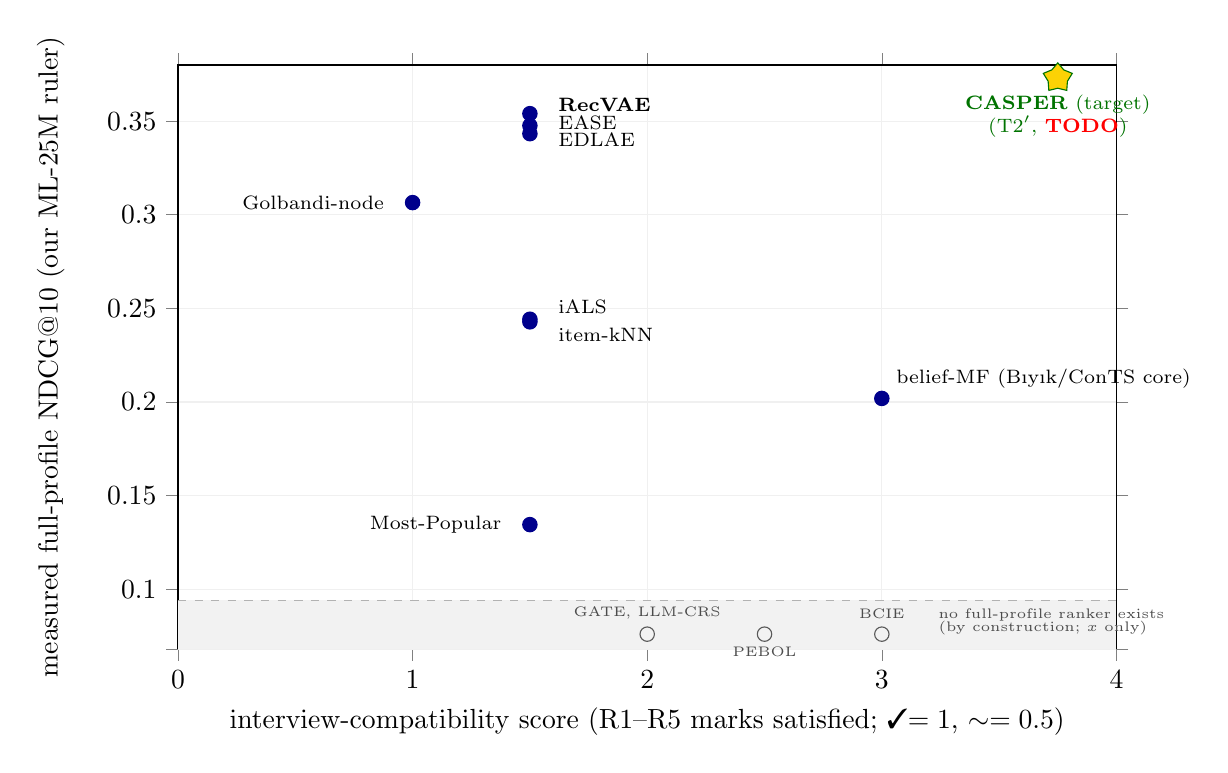
\begin{tikzpicture}
\begin{axis}[
    width=13.5cm, height=9cm,
    xlabel={interview-compatibility score (R1--R5 marks satisfied; \cmark$=1$, \pmark$=0.5$)},
    ylabel={measured full-profile NDCG@10 (our ML-25M ruler)},
    xmin=0, xmax=4, ymin=0.068, ymax=0.38,
    xtick={0,1,2,3,4},
    ytick={0.10,0.15,0.20,0.25,0.30,0.35},
    ymajorgrids=true,
    extra y ticks={0.068}, extra y tick labels={},
    grid=both, grid style={gray!12},
    axis line style={-Latex},
    tick align=outside,
    clip=false,
]
  % --- target: star only (author preference; no box) ---
  \node[star,star points=5,draw=green!45!black,fill=yellow!85!red,minimum size=11pt,inner sep=0pt]
        at (axis cs:3.75,0.373) {};
  \node[green!45!black,font=\scriptsize,align=center,anchor=north] at (axis cs:3.75,0.369)
        {\textbf{CASPER} (target)\\(T2$'$, \textcolor{red}{\textbf{TODO}})};
  % --- measured points (filled); x = R2..R5 marks ONLY (R1 excluded: accuracy is the y-axis) ---
  \addplot[only marks,mark=*,mark size=2.6pt,color=blue!55!black] coordinates {
    (1.5,0.1345) (1.5,0.2428) (1.5,0.2442) (3.0,0.2019)
    (1.0,0.3065) (1.5,0.3433) (1.5,0.3476) (1.5,0.3540)
  };
  % measured-point labels (accuracy cluster stacked at x=1.5, spread by y)
  \node[font=\scriptsize,anchor=east] at (axis cs:1.42,0.1345) {Most-Popular};
  \node[font=\scriptsize,anchor=west] at (axis cs:1.58,0.2360) {item-kNN};
  \node[font=\scriptsize,anchor=west] at (axis cs:1.58,0.2510) {iALS};
  \node[font=\scriptsize,anchor=east] at (axis cs:0.92,0.3065) {Golbandi-node};
  \node[font=\scriptsize,anchor=west] at (axis cs:1.58,0.3400) {EDLAE};
  \node[font=\scriptsize,anchor=west] at (axis cs:1.58,0.3490) {EASE};
  \node[font=\scriptsize,anchor=west] at (axis cs:1.58,0.3585) {\textbf{RecVAE}};
  \node[font=\scriptsize,anchor=south west] at (axis cs:3.02,0.2019) {belief-MF (B\i y\i k/ConTS core)};
  % --- "no full-profile number" strip: BELOW the measured y-scale, visually separated ---
  \fill[gray!10] (axis cs:0,0.068) rectangle (axis cs:4,0.094);
  \draw[gray!60,dashed] (axis cs:0,0.094) -- (axis cs:4,0.094);
  \addplot[only marks,mark=o,mark size=2.6pt,color=gray!70!black] coordinates {
    (2.0,0.076) (2.5,0.076) (3.0,0.076)
  };
  \node[gray!60!black,font=\tiny,anchor=south] at (axis cs:2.0,0.079) {GATE, LLM-CRS};
  \node[gray!60!black,font=\tiny,anchor=north] at (axis cs:2.5,0.0745) {PEBOL};
  \node[gray!60!black,font=\tiny,anchor=south] at (axis cs:3.0,0.079) {BCIE};
  \node[gray!60!black,font=\tiny,anchor=west] at (axis cs:3.20,0.086)
        {no full-profile ranker exists};
  \node[gray!60!black,font=\tiny,anchor=west] at (axis cs:3.20,0.079)
        {(by construction; $x$ only)};
\end{axis}
\end{tikzpicture}
\caption{\textbf{The gap map (measured axes).} $y$-axis: measured full-profile NDCG@10 on our canonical ML-25M ruler.
$x$-axis: an \emph{interview-compatibility score}, defined as the number of \textbf{R2--R5} marks a system carries in
the master table (Table~\ref{tab:master}), scoring \cmark${=}1$ and \pmark${=}0.5$, maximum $4$. \emph{R1 is
deliberately excluded from the score}: accuracy is the $y$-axis, and letting it also inflate $x$ would blur the very
trade-off the figure exists to show. The score is a \emph{coarse ordinal capability count, not a measurement}, so the
$x$-axis is qualitative even though the $y$-axis is measured. Filled markers are systems with a full-profile number on
this ruler (belief-MF is the shared B\i y\i k/ConTS posterior core; Golbandi-node is the tree's best-effort node
recommender). Hollow markers in the separated grey strip \emph{below} the measured $y$-scale are systems that
\emph{cannot produce a full-profile number by construction} (no full-catalogue ranker, or not portable; see the
master-table dispositions); only their $x$ position is meaningful. Runnable-but-not-yet-measured systems (sequence
models, graph filters, EDDI, TaNP) are deliberately \emph{absent} from the figure --- they carry \TODO{} cells in
Table~\ref{tab:master} and join the plot when their numbers land. The star marks the instrument target (high compatibility at
the frontier bar), still \TODO{}. The population is \emph{bimodal}: the entire accuracy corner
(Pop through RecVAE, $0.343$--$0.354$ at the top) collapses onto $x\le1.5$---strong recommenders that can fold items
and nothing else---while every system with genuine interview machinery sits at $x\ge2$ and either has no measurable
full-profile accuracy at all (the grey strip) or, for the one measurable core, drops to $0.2019$, below plain matrix
factorisation (belief-MF at $x{=}3$). Two clusters, no bridge: the corner is not expensive; it is unoccupied. The
nearest published rival to the target is B\i y\i k et al.~\cite{biyik2023soft} (highest compatibility of any system
with an actionable belief), whose runnable core nonetheless measures far below the frontier bar.}
\label{fig:gapmap}
\end{figure}

% =====================================================================
\section{Gap analysis}\label{sec:gap}
% =====================================================================

\paragraph{The verdict.}
No single published system satisfies all of $\{$R1 SOTA-full-profile $\wedge$ R2 any-length set $\wedge$ R3
channel-agnostic via arbitrary embeddings $\wedge$ R4 uncertainty-native $\wedge$ R5 monotone$\}$. The binding
near-miss is Bıyık et al.~\cite{biyik2023soft}: it fails R1 (a co-trained item space, not a frozen certified
RecVAE-class tower, and no full-profile benchmark) and gives only an approximate, ``generally not Gaussian''
posterior; every other candidate fails R3 or R4 outright. \textbf{We are aware of none} that occupies the
conjunction---and we state it exactly that way, never as ``there is none.''

\paragraph{Per-near-miss failure analysis.}
\begin{itemize}[leftmargin=1.4em,itemsep=2pt]
  \item \textbf{Bıyık et al.~2023}~\cite{biyik2023soft} --- has R2 $+$ R3 (items and soft attributes as directions)
        $+$ R4 (Gaussian belief). \emph{Fails R1}: the item space is co-trained with the belief model, not a certified
        full-profile CF tower, and accuracy is reported on their elicitation task, not the EASE/RecVAE bar. R3 is
        \emph{attribute directions}, not arbitrary embeddings / open concepts / continuous query tokens. R5 is
        approximate (sampled EVOI over a non-Gaussian posterior). This is the central threat, and our wedge is exactly
        (a) frozen certified tower vs.\ co-trained, (b) exact conjugacy vs.\ approximate posterior, (c) arbitrary /
        open / continuous tokens vs.\ a fixed attribute set.
  \item \textbf{ConTS}~\cite{li2021seamlessly} --- R2 $+$ R4 $+$ a unified item/attribute action space.
        \emph{Fails R3} (a fixed categorical attribute schema; no arbitrary embedding, no continuous or open token) and
        \emph{R1} (a bandit over arms, not a full-profile encoder).
  \item \textbf{EDDI / Partial-VAE}~\cite{ma2019eddi} --- R2 $+$ R4 (information-gain) $+$ set input.
        \emph{Fails R1} (not a recommendation model / no CF SOTA) and \emph{R3} (no attribute or concept channel as
        demonstrated).
  \item \textbf{RecVAE / EASE}~\cite{ren2020recvae,steck2019ease} --- \emph{R1 yes.} \emph{Fail R3} (an item-only
        one-hot / indicator basis---cannot express a concept, a signed value, or a continuous direction) and \emph{R4}
        (point estimate; RecVAE's latent posterior is item-only and is not used as an actionable belief).
  \item \textbf{PEBOL}~\cite{austin2024bayesian} --- R4 (per-item Beta) $+$ R3 (LLM aspects) $+$ strong cold-start.
        \emph{Fails R1} (no full-profile CF ranking) and its R4 is \emph{per item}, not a shared user covariance; no
        monotonicity guarantee.
  \item \textbf{SASRec / BERT4Rec}~\cite{kang2018sasrec,sun2019bert4rec} --- R2 (re-encode the sequence).
        \emph{Fail R3, R4, R5} (item-only, order-sensitive, point estimate, non-monotone---a later token can reorder
        everything). Token input is trivially satisfied but is \emph{not} value-carrying or mixed-type, so ``interview
        $=$ tokens'' does not hold; and BERT4Rec's fold-in advantage carries a replicability
        caveat~\cite{petrov2022replicability}.
\end{itemize}

\paragraph{The three inexpressible legs.}
Three input channels are \emph{architecturally impossible} (not merely untuned) in the item-indicator basis of every
R1-bar model: (i) graded/signed per-entity values (the basis has no sign and no magnitude---a ``dislike'' is not
representable as a negative one-hot without changing the likelihood), (ii) out-of-catalogue concepts (there is no
column for an entity absent from the catalogue), and (iii) arbitrary continuous direction tokens. Folding these as
\emph{linear observations in a frozen latent} is the one leg of the conjunction we find nowhere in the literature.

\paragraph{Pre-empted---cited, never claimed as first.}
We must credit, and do not claim priority over: attribute-answers-as-directions plus a Bayesian
fold~\cite{biyik2023soft}; unified item$+$attribute belief and value-of-information~\cite{biyik2023soft,li2021seamlessly};
conjugate-Gaussian folds over a frozen factorisation~\cite{toroghi2023bcie}; permutation-invariant set-encoders with
information-gain acquisition~\cite{ma2019eddi}; value-carrying set-input cold-start recommenders~\cite{lin2021tanp};
the non-degradation-of-information principle (Good 1967 / Blackwell); and the now-crowded ``uncertainty-native
recommender'' area~\cite{wang2025bdecf}. Our defensible novelty is only the \emph{conjunction} of all five requirements
in one frozen certified tower, plus the three inexpressible legs and the G0--G2 protocol.

% =====================================================================
\section{The instrument}\label{sec:method}
% =====================================================================

The design follows directly from the gap analysis: use the shallow frozen tower that already holds the accuracy
corner (R1, and the flat-since-2019 frontier means no deep-net detour is warranted), and add the one belief mechanism
with a principled monotonicity story---exact linear-Gaussian conjugacy---over its frozen latent (R4, R5), with a
channel-agnostic linear-observation interface (R3). This section is written at design level; implementation details
and all numbers are \TODO{}.

\subsection{Frozen shallow-SOTA tower}
The substrate is a certified shallow recommender---a RecVAE-class amortised encoder or a closed-form
autoencoder~\cite{ren2020recvae,steck2019ease}---trained once on the full catalogue and then \emph{frozen}. It exposes
(a) item factor rows $\Q_i\in\R^{d}$, (b) a decoder read-out $s_i(\uu)=\Q_i^\top\uu + \beta_i$ with a learned bias
$\beta_i$, and (c) the encoder that maps a full interaction set to a latent. Freezing is the wedge against
Bıyık~\cite{biyik2023soft} (co-trained) and the guarantee that G0 (full strength preserved) is a property of the
substrate, not of the belief layer. We deliberately do \emph{not} extend the linear basis with concept columns
(that stays in the item-indicator world and fails R3), nor learn the uncertainty head (no monotonicity story, and
retraining risks G0). \TODO{Select and certify the frozen tower (paper-config RecVAE candidate at $0.3540/0.2497$;
report the certified full/tail NDCG@10 and the bridge number of \S\ref{sec:bridge}).}

\subsection{Analytic conjugate-Gaussian belief layer}
Over the frozen latent we place a Gaussian belief on the user vector, $\uu\sim\mathcal N(\bmu_0,\bSigma_0)$, and model
each answer as a noisy linear read-out along the queried direction:
\begin{equation}\label{eq:obs}
  y_j \;=\; \bphi_j^\top\uu + \varepsilon_j,\qquad \varepsilon_j\sim\mathcal N(0,\sigma_j^2).
\end{equation}
Because the observation is linear-Gaussian, the posterior after $\mathcal E_t$ is Gaussian in closed form; maintaining
it in \emph{precision} form (a precision accumulator) makes the any-length fold-in a single running sum:
\begin{equation}\label{eq:precacc}
  \bLambda_t \;=\; \bLambda_0 + \sum_{j=1}^{t}\sigma_j^{-2}\,\bphi_j\bphi_j^\top,\qquad
  \bLambda_t\,\bmu_t \;=\; \bLambda_0\bmu_0 + \sum_{j=1}^{t}\sigma_j^{-2}\,y_j\,\bphi_j,\qquad
  \bSigma_t=\bLambda_t^{-1}.
\end{equation}
Equation~\eqref{eq:precacc} is exactly the mechanism BCIE~\cite{toroghi2023bcie} uses for critiques over a frozen
factorisation; our contribution is doing it over a \emph{certified full-profile SOTA} tower with channel-agnostic
tokens, and certifying the G0--G2 protocol on it. Three properties fall out by construction: it is a permutation-invariant
\emph{set} operation defined for every $t\ge 0$ (R2); each update adds a rank-1 term along $\bphi_{t+1}$, so
$\bLambda_t$ only grows and $\det\bSigma_t$ only shrinks (G1); and conjugate updates are Blackwell/Good-1967 monotone
in \emph{expected utility}. The last is why R5 is plausible, but---because the tower's dot-product ranker does not act
optimally under the belief---per-question NDCG monotonicity is \emph{not} automatic and must be shown empirically
(\S\ref{sec:limits}). \TODO{Fix $\bLambda_0,\bmu_0$ (prior from the tower), the per-channel noise $\sigma_j$, and the
confidence/temperature schedule; verify G0 holds at the belief mean on the full profile.}

\subsection{Channel-agnostic tokens as linear observations}
Every channel supplies a direction $\bphi_j\in\R^{d}$ and a value $y_j\in\R$ to Eq.~\eqref{eq:precacc}; the update is
identical across channels (R3):
\begin{itemize}[leftmargin=1.4em,itemsep=1.5pt]
  \item \textbf{Items.} $\bphi_j=\Q_i$ (the frozen item factor). A graded or signed answer sets $y_j$; a dislike is a
        negative $y_j$ along the same direction---representable here precisely because the observation model
        \eqref{eq:obs} has a sign and a magnitude, unlike a one-hot indicator.
  \item \textbf{Out-of-catalogue concepts.} $\bphi_j$ is a concept direction in the latent (e.g.\ a centroid of member
        factors, or a text-adapter image of the concept), folded exactly like an item---no catalogue column required.
  \item \textbf{Entities / free text.} An embedding is projected into the latent by a fixed adapter and folded
        identically.
  \item \textbf{Continuous direction tokens.} A policy may emit any $\bphi_j\in\R^{d}$ directly (the continuous-action
        interface the companion chapter uses); the belief update does not distinguish it from a catalogue entity.
\end{itemize}
The signed/graded, out-of-catalogue, and continuous legs are the three channels inexpressible in the R1-bar basis
(\S\ref{sec:gap}). \TODO{Specify the concept-direction and text-adapter constructions, the polarity/gradation
encoding, and the acceptance tests (a like/dislike flip reverses the queried neighbourhood; a concept fold lifts its
member items; monotone in $t$).}

\begin{figure}[t]
  \centering
  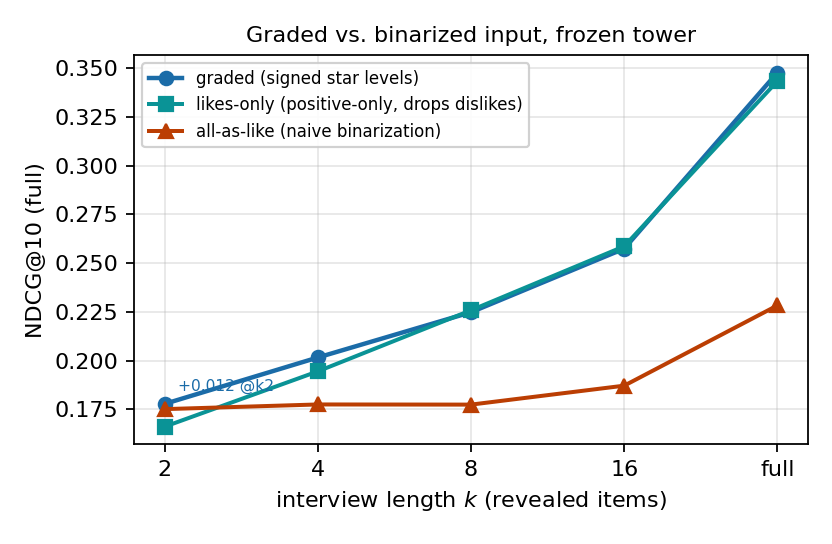
\includegraphics[width=0.62\linewidth]{fig_graded_curve.png}
  \caption{\textbf{The signed/graded leg, empirically (provisional; frozen graded-native tower, ML-25M
    interview harness, VAL, full NDCG@10 vs.\ interview length $k$).} The same revealed set is fed three ways.
    \emph{Graded} (real signed star levels) and \emph{likes-only} (sub-threshold answers dropped---what a
    positive-only tower such as RecVAE does at $r{>}3.5$) nearly coincide: the fine gradations add only a small,
    short-interview premium over likes-only ($+0.012$ at $k{=}2$, fading to $\approx 0$ by $k{=}8$; CI-clean).
    Both dominate \emph{all-as-like} (every answered item recorded as a $4$-star like---naive implicit
    binarization), which stays flat and low because it \emph{mislabels dislikes as likes}; that gap widens with
    $k$ ($-0.12$ at full profile) as more dislikes are corrupted. The leg's value is thus \emph{representing a
    dislike at all}---a negative $y_j$ the item-indicator basis cannot encode---rather than fine gradation among
    likes; mirroring the star signs (flip control) costs $-0.29$ at full profile. \emph{Provisional pending the
    certified tower (\S\ref{sec:expdesign}).}}
  \label{fig:gradedcurve}
\end{figure}

% =====================================================================
\section{The concept channel: derivation, lineage, and failure analysis}\label{sec:concept}
% =====================================================================

The out-of-catalogue concept leg is the most demanding of the three inexpressible channels---it is the one with no
catalogue column, no interaction count, and no sign in the item-indicator basis---so we work it out in full. Three
things must be made concrete: how a concept answer becomes an observation pair $(\bphi_c, y_c)$ for the belief update
of Eq.~\eqref{eq:precacc}; where each piece sits in the published record (so that we claim only the conjunction, never
a component); and---because the honest history of this channel includes a self-inflicted regression---what a measured
failure of our \emph{own} evaluation harness taught us about which gate class the battery was missing. This section
is written at derivation level; the concept-channel numbers below are measured on the internal ML-25M interview
harness and are reported as such, while the certified instrument curves remain \TODO{} (\S\ref{sec:expdesign}).

\subsection{A signed, exposure-corrected affinity estimator}\label{sec:concept:est}

A concept answer must supply the value $y_c$ that Eq.~\eqref{eq:obs} reads along the concept direction. We want that
value to be \emph{signed} (a user can dislike ``horror,'' not merely fail to like it), \emph{popularity-corrected} (a
concept made of blockbusters must not read as universal affinity), \emph{volume-corrected} (a heavy watcher must not
read as liking everything), and \emph{confidence-bearing} (a concept the user has plausibly never been exposed to is a
\emph{refusal}, not a dislike). Two estimators, an implicit and an explicit one, combine to meet this.

Let $\mathcal I_u$ be the user's watched set, $p_i$ the catalogue marginal of item $i$, and let concept $c$ have member
set $M_c$. Write $n_c=|\mathcal I_u\cap M_c|$ for the user's watched members and $e_c=|\mathcal I_u|\cdot\pi_c$ for the
number \emph{expected} under the user's volume times the concept's popularity $\pi_c=\sum_{i\in M_c}p_i$. The implicit
\emph{selection} estimator is the add-$\tfrac12$ log watch-lift
\begin{equation}\label{eq:sel}
  \mathrm{SEL}(u,c) \;=\; \log_2\frac{n_c+0.5}{e_c+0.5}
  \;\;\approx\;\; \mathrm{PMI}(u,c),
\end{equation}
which is precisely the \emph{pointwise mutual information} between the user and the concept: the denominator's $\pi_c$
divides out concept popularity, and forming $e_c$ from the user's own volume divides out user activity, so SEL is
positive for genuine affinity, near zero for popularity-explained co-occurrence, and \emph{negative for avoidance}.
Its normalised form is the NPMI, $\mathrm{NPMI}=\mathrm{PMI}/(-\log_2 \hat p_{uc})\in[-1,1]$, which tames PMI's
small-count inflation and yields a bounded, comparable score. The explicit \emph{value} estimator is a support-shrunk
signed rating residual,
\begin{equation}\label{eq:val}
  \mathrm{VAL}(u,c) \;=\; \frac{n_c}{n_c+\lambda}\;\bar r^{\,\mathrm{res}}_{uc},
  \qquad \lambda=3,\qquad
  \bar r^{\,\mathrm{res}}_{uc}=\frac{1}{n_c}\!\!\sum_{i\in\mathcal I_u\cap M_c}\!\!\bigl(r_{ui}-\bar r_i\bigr),
\end{equation}
the mean rating the user gives the concept's members \emph{above each item's own mean}, shrunk toward zero by the
Beta-style factor $n_c/(n_c+\lambda)$ so that a one-film opinion counts for little. Both estimators are signed and
combine into a four-band answer: a \emph{graded like} (SEL/VAL band above the neutral zone), a \emph{neutral}
(indistinguishable-from-exposure), a \emph{graded dislike} (band below), and a \emph{refusal} issued exactly when the
expected support falls below a threshold, $e_c<\tau$, i.e.\ when the user has plausibly never been exposed to the
concept and no answer should be forced.

\paragraph{Lineage.} Every piece is established prior art, which is the point of stating it explicitly. The log-lift
\eqref{eq:sel} is PMI/NPMI, the standard popularity-corrected association score. Reading a \emph{magnitude} of implicit
consumption as evidence is Hu--Koren--Volinsky's implicit-confidence template~\cite{hu2008collaborative}---except that
HKV lets the count re-enter \emph{only as a loss confidence weight, never as a sign}, which is exactly the assumption
our signed estimator breaks. The principled account of why a non-watch is not a dislike is
ExpoMF~\cite{liang2016expomf}: it separates a latent \emph{exposure} variable (was the user even aware of the item)
from \emph{preference}, so that non-consumption is modelled as ``not exposed'' \emph{or} ``exposed-and-disliked''---the
generative gold standard our refusal band ($e_c<\tau$) and popularity-corrected $e_c$ approximate cheaply and in closed
form. The unbiased-learning route to the same correction is attribute-level exposure
propensity~\cite{qin2020attributepropensity}, which IPS-reweights implicit feedback by a per-attribute propensity;
it is the heavier, variance-prone alternative to our moment estimator. Finally, calibrated
recommendation~\cite{steck2018calibrated} builds a user's normalised genre \emph{distribution} $p(g\mid u)$---the
closest widely-used ``concept profile,'' but a distribution that sums to one and therefore encodes relative emphasis
only: it \emph{cannot express dislike}, which is precisely the expressive gap SEL$<0$ fills.

\paragraph{Why the implicit channel, quantified.} On an informativeness decomposition (a per-concept linear fit of the
oracle concept affinity onto each candidate answer, $R^2$), the implicit watch-lift dominates: SEL explains $0.376$ of
the affinity variance, the explicit rating residual VAL a further $+0.042$ (SEL$+$VAL $0.398$), while an LLM-elicited
ordinal answer explains only $0.017$ (an internal decomposition)---implicit outperforms the explicit LLM answer by
roughly $22\times$.
Because SEL is built from raw watch counts and item marginals, it uses no recommender geometry, so this signal is
\emph{non-circular by construction} (it even beats a model-geometry projection of the same residuals). This is the
evidence that the concept channel's value is worth carrying signed rather than as a mere membership indicator; the
decomposition is an informativeness measurement, not an interview curve, and is reported as such.

\subsection{The fold operator: whitened directions and a gated fold-to-point}\label{sec:concept:fold}

The direction $\bphi_c$ must point where the concept's taste lives, not where popularity lives. A raw member centroid
fails this: a shared popularity component (random concept pairs have cosine $\approx 0.5$) masks the genre geometry.
Removing it---centre the member factors and strip the top-1 principal component (the popularity axis), the
all-but-the-top whitening of Mu and Viswanath---turns the centroid into a usable direction: concept-membership
discrimination through the frozen decoder rises from AUC $0.44$ (raw, at chance) to $0.94$ (whitened). We therefore
take $\bphi_c$ to be the \emph{whitened member centroid}, IDF-weighted by $1/\log(1+|M_c|)$ so broad genres do not
dominate. Whitening is a fix, not a contribution, and is cited as such.

The operator that consumes $(\bphi_c,y_c)$ is where the design decision lives, and our own history is a clean
ablation between two families. An \emph{additive-union} operator scores each item by summing concept contributions on
a popularity floor, $s_i=\beta_i+\sum_c w_c\,\langle \W_d\Q_i,\bphi_c\rangle$. It has the right monotonicity floor (an
empty interview scores exactly $\beta_i$) but the wrong composition: it scores the \emph{union} of directions, so
correlated sibling concepts (``dark,'' ``gritty,'' ``noir'') re-add the same acclaim axis and over-count. Measured
against a no-answer intercept of $0.1279$ full NDCG@10, the additive channel peaks early (about $+0.011$ at two
answers) and then \emph{craters} as answers accumulate, reaching $0.0991$ at eight answers---below the intercept. A
\emph{trained gated fold-to-point} operator fixes this by folding the answers into the latent itself and letting a
frozen decoder apply the full collaborative (intersection) structure:
\begin{equation}\label{eq:cfold}
  \uu \;\leftarrow\; \uu + \sigma\!\bigl(g([\uu;\bphi_c;y_c])\bigr)\;\odot\;h([\uu;\bphi_c;y_c]),
\end{equation}
with the gate $g$ and the delta MLP $h$ \emph{zero-initialised} (so at initialisation $\uu$ is unchanged and G0
survives) and the accumulated shift norm-capped per user. This operator is monotone in the number of answers to eight
(concepts-only $0.2091/0.1222$ full/tail at eight answers, up from the $0.1717$ cold point) and, crucially,
\emph{redundancy-robust}: feeding it eight \emph{correlated} top-SEL concepts still reaches $0.2219$ full, at or above
its four-answer level, where the additive-union operator degraded. The gated fold is the concept operator we adopt;
Eq.~\eqref{eq:cfold} is the concept-channel instantiation of the linear-observation fold, with the belief covariance
maintained analytically as in \S\ref{sec:method}.

\paragraph{Lineage.} The skeleton---an attribute as a latent direction, folded by a Bayesian belief update over a
frozen factor space---is well-trodden, and we claim none of it in isolation. Bıyık et al.~\cite{biyik2023soft} treat a
soft attribute as a concept-activation-vector direction and fold signed answers into a Gaussian belief; M\&Ms-VAE
folds a rating-posterior and an attribute-posterior over one latent by a product-of-experts
merge~\cite{antognini2021mmvae}; its successor adds an independent \emph{signed} critique axis through learned
positive/negative conditioning tokens, and reports that negative critiquing saturates after about five
turns~\cite{antognini2022posneg}---a concrete ceiling for any signed-attribute channel, consistent with our own
front-loaded concept curves. BK-VAE folds keyphrase-activation-vector directions by a Bayesian critiquing
step~\cite{luo2021bkvae}; the gate/MLP of Eq.~\eqref{eq:cfold} is a per-token generalisation of FiLM
conditioning~\cite{perez2018film}, which a single global affine cannot do because it would apply the same modulation to
item and concept tokens alike. And the decision to \emph{freeze} the tower rather than co-train a concept head is a
direct reading of the cautionary result that a bolt-on critique head costs recommendation
accuracy~\cite{luo2019deepcritiquing}. What none of these holds jointly---and what we are aware of no system holding---is
the conjunction this channel occupies: \emph{continuous, out-of-catalogue concept directions} (a whitened centroid, or
a text-adapter image, with no per-attribute probe to train), driven by a \emph{signed, exposure-corrected implicit
affinity} (Eqs.~\eqref{eq:sel}--\eqref{eq:val}), folded over a \emph{frozen, certified full-profile SOTA tower}. The
components are borrowed; only their conjunction is claimed.

\subsection{Failure analysis: a positive-only clip and the deployment-currency gate}\label{sec:concept:fail}

The honest history of this channel includes a regression we introduced ourselves, and it is worth recording because it
exposes a whole \emph{class} of gate the battery originally lacked. When the concept curves were first built, the
evaluation harness clipped every folded concept value to $[0.25,1]$---the like-levels only---silently discarding the
negative half of the estimator that \S\ref{sec:concept:est} works so hard to produce. Selection kept only
positive-lift concepts and floored the survivors at a weak positive; SEL$<0$ was \emph{computed and then thrown away}.

The consequence only became visible in the right currency. Per-answer curves that privilege each user's own top-SEL
concepts looked fine, but those are unknowable before the interview. Measured in \emph{deployment currency}---a
realizable, generic question bank with a per-question budget, where most answers down a fixed bank are weak
positives---the accumulated weak-positive ``poison'' dragged the ranking \emph{below the no-answer intercept}:
concepts-only full NDCG@10 declined from $0.1304$ to $0.1160$ by the sixteenth question, under the $0.1279$ intercept.
The channel was structurally unable to say ``no,'' even though the fold operator of Eq.~\eqref{eq:cfold} is
\emph{sign-capable}---a flip test on it moves NDCG by $-0.201$ with a clean CI. That is the crux: \textbf{a capability
gate is vacuous if the answer model never exercises the capability.} The sign-flip gate (G3) passed on a channel that,
as actually driven in deployment, never emitted a negative answer at all.

We close this with a pre-registered, eval-only triple gate (recorded as the signed-SEL gate specification) that a
retrain must clear before the signed answer is adopted:
\begin{enumerate}[leftmargin=1.6em,itemsep=1.5pt]
  \item \textbf{Recovery.} Signed answers routed through the sign-capable operator recover $+0.0076$ full NDCG@10 at
        the sixteenth question with a CI excluding zero, and about $1.5\times$ the tail---turning the deployment decline
        into a gain.
  \item \textbf{Counterfeit control (taste, not artifact).} An adversarial review flagged that ``dislike from absence''
        could be a volume$\times$popularity artifact; a counterfeit answer built only from user volume and concept
        popularity reproduces \emph{zero} of the recovery, so the gain is taste, not an exposure artifact.
  \item \textbf{Out-of-curriculum control.} A meh-only control shows the residual late decline is out-of-curriculum
        extrapolation---the operator was trained on interviews of up to eight answers and asked sixteen---rather than a
        sign defect, isolating the two failure modes.
\end{enumerate}
Because ``dislike from absence'' can leak user volume into the belief, we pair the gate with a volume-invariance
acceptance criterion, backed by a probe: the recoverability of log watch-volume from the belief latent
($R^2$ of a linear read-out) rises from $0.025$ to $0.204$ once signed answers are folded, so a signed-answer build is
accepted only if that leak is held down (a volume-orthogonalised fold, or an invariance penalty).

\paragraph{The lesson for the battery.} The outcome-gate false positives of \S\ref{sec:reqs} have a sibling among the
\emph{semantic} gates. A capability gate such as G3's sign-flip certifies that the operator \emph{can} negate; it says
nothing about whether the operator, driven by a realistic answer model down a realistic question bank, ever \emph{does}.
The miss is closed only by a \emph{deployment-currency} gate---evaluate the channel on a fixed, user-independent
question bank under a per-question budget (the G9 ingestion-isolation setting, scored at the endpoint), where an
answer model that never exercises the negative half is penalised by the same declining curve that exposed the clip.
We therefore add the deployment-currency endpoint as the acceptance form of the concept channel: not ``can the operator
express dislike'' but ``does the realizable interview stay above the no-answer intercept at budget.''

\subsection{Results: the signed retrain, and where the concept channel wins}\label{sec:concept:results}

The signed retrain of \S\ref{sec:concept:fail} has since landed, and we ran the two channels---concepts and
items---through \emph{one} deployment-currency harness (10{,}000 held-out cold users, per-question budget, every
question spending budget whether answered or not, scored on full \emph{and} tail NDCG@10 against the no-answer
intercept $0.1279/0.0192$). The results are reported here on the internal ML-25M interview harness; the certified
instrument curves remain \TODO{} (\S\ref{sec:expdesign}). They tell a consistent, and deliberately un-triumphal,
story: the signed answer repairs the regression, but the concept channel's value is \emph{shaped}---it owns the
opening of an interview and cedes the long tail of it to items---and its largest prize is one we do not yet capture.

\paragraph{The signed answer turns the deployment decline into a gain.} Re-running the pre-registered triple gate on
the \emph{retrained} model (not merely the eval-only fold of \S\ref{sec:concept:fail}) clears all three taste
criteria. Signed answers beat the positive-only clip by $+0.0104$ full NDCG@10 at the sixteenth question (CI
$[+0.0075,+0.0134]$): the clip-up curve sinks below the intercept by the eighth question and stays there ($0.1268$ at
$q{=}16$), while the signed curve holds above it ($0.1372$). The counterfeit control---an answer built only from user
volume and concept popularity---reproduces \emph{none} of the gain (it declines, $-0.045$ at $q{=}16$), so the signal
is taste, not a volume$\times$popularity artifact; and permuting the answer values across concepts collapses the gain
($+0.0335$ CI-excluding-zero relative to the permutation), so it is the answer \emph{values} that carry it, not fold
cardinality. \emph{One acceptance criterion remains unmet, and we record it plainly:} the volume-invariance gate still
fails. The recoverability of log watch-volume from the belief latent is $R^2\,0.249$ after the retrain, against a
pre-registered bar of $\le 0.05$---the per-user negative-channel cap did not hold the leak down. We treat the signed
concept answer as \emph{directionally supported but not yet certified}: the counterfeit-clean result is the
waiver-consideration evidence (the leaked quantity is user volume, but the ranking gain provably is not a volume
meter), and the fold's acceptance is pending either a volume-orthogonalised variant or an author ruling on the waiver.

\begin{figure}[t]\centering
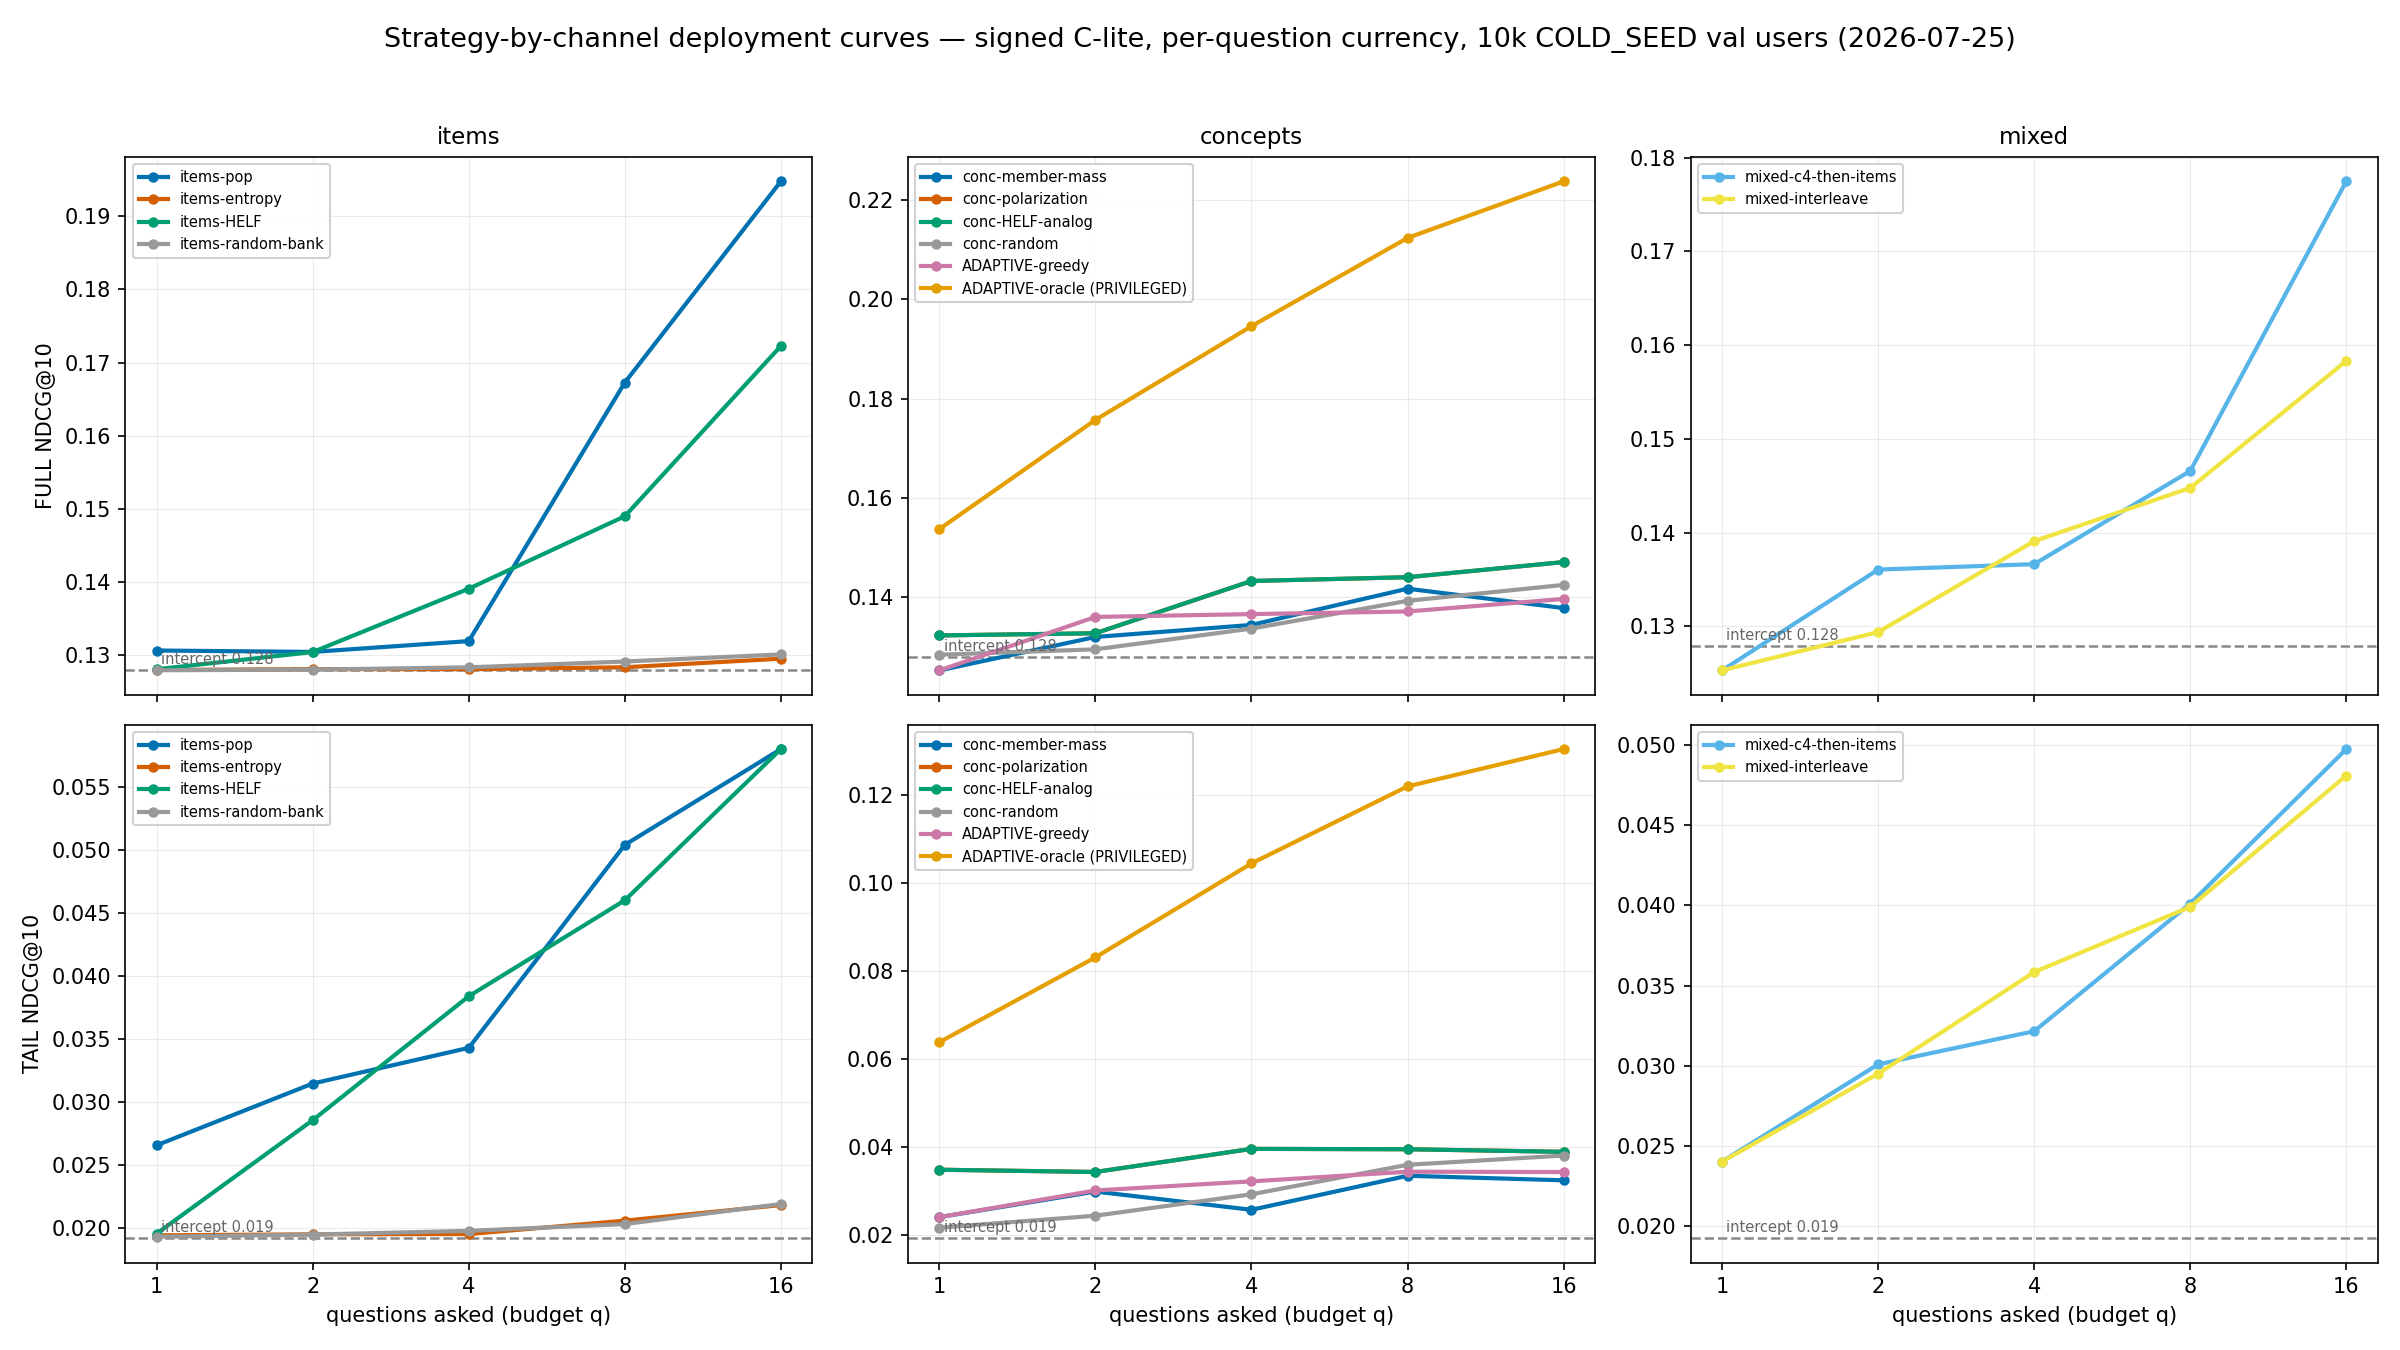
\includegraphics[width=\linewidth]{fig_strategy_channel_suite.png}
\caption{\textbf{Strategy $\times$ channel deployment suite} (internal ML-25M interview harness, 10k cold users,
per-question budget; signed C-lite as the fold). Full and tail NDCG@10 versus the number of questions, for item-side
question strategies (popularity, HELF, entropy, random bank), concept-side strategies (polarization/HELF-analog,
member-mass, random), static mixes, the realizable adaptive greedy selector, and the privileged adaptive oracle,
against the no-answer intercept. \emph{Concepts own the short interview} (a polarizing-concept opener is the best
single question on both metrics, and concept strategies lead every item strategy through $q{\approx}4$); \emph{items
win the long interview} (popularity-ranked items are highest from $q{=}8$ onward); \emph{static mixes underperform
pure items past $q{=}8$}; and the \emph{privileged oracle} sits far above every realizable arm at all budgets, while
the realizable greedy selector recovers only a small single-digit fraction of that oracle$-$static gap---the large,
unclaimed adaptive prize that motivates the companion method chapter. All curves are \TODO{} pending the certified
tower.}
\label{fig:strategychannel}
\end{figure}

\paragraph{Concepts own the short interview; items win the long one.} Figure~\ref{fig:strategychannel} is the headline
picture. Reading it against the intercept: the single most informative \emph{opening} question is a \emph{polarizing
concept}---the polarization-ranked concept strategy reaches $0.1323/0.0348$ (full/tail) after one question, above the
best item strategy's $0.1307/0.0266$ (popularity-ranked items) on \emph{both} metrics, and concept strategies stay
ahead of every item strategy through about the fourth question ($0.1433/0.0395$ for polarizing concepts at $q{=}4$
versus $0.1391/0.0384$ for the best item strategy, HELF). This is the coarse-to-fine intuition made concrete: a good
first move splits a cold population along a taste axis, and a concept does that in one question where an item barely
moves the belief. But the advantage is front-loaded. From the eighth question onward, popularity-ranked \emph{items}
are the strongest realizable arm ($0.1673/0.0504$ at $q{=}8$, $0.1948/0.0580$ at $q{=}16$), while the best concept
strategy plateaus near $0.1471/0.0389$---the coarse concept direction localises the belief but cannot keep refining it,
exactly the front-loaded-then-plateau ceiling the signed-critiquing literature reports at about five
turns~\cite{antognini2022posneg}. Static \emph{mixed} schedules do not rescue the long interview: a coarse-to-fine mix
(concepts first, then items) trails pure popularity items past $q{=}8$ ($0.1775$ versus $0.1948$ at $q{=}16$). The
operational reading is that concepts are a short-interview and cold-open instrument, not an item replacement---which is
what the coarseness ceiling predicted.

\paragraph{The adaptive prize is large and unclaimed.} The privileged \emph{oracle} selector---which sees each user's
own most informative next question---sits far above every realizable arm at every budget ($0.2237/0.1305$ at $q{=}16$,
against popularity items' $0.1948/0.0580$), and the oracle$-$static gap widens with budget (full gap $0.086$, tail
$0.098$ at $q{=}16$). A realizable greedy selector on this same harness recovers only a small single-digit fraction of
that gap ($2.1\%$ full, $1.9\%$ tail at $q{=}16$, and \emph{negative} at $q{=}8$, where it does not even beat the
static member-mass concept order, $-0.0046$ full, CI-clean). We flag this as a positive finding for the companion
chapter rather than a defeat here: a large adaptive headroom that a naive greedy policy cannot capture is precisely the
regime a learned selector should address---the decision-tree acquisition line of Golbandi et
al.~\cite{golbandi2011adaptive} on \emph{this} instrument and harness. The instrument chapter's job is to make the
gap \emph{measurable}; closing it is the method chapter's.

\paragraph{Training concepts into the tower is item-safe but buys nothing.} We evaluated two homes for the signed
concept fold: a trained fold-to-point on the \emph{frozen} tower (call it the frozen-fold), and concept tokens trained
\emph{into} the tower itself (the tokens-in-tower variant). Both preserve full-profile strength, as G0 demands. The
frozen-fold inherits the tower's G0 by construction (a zero-initialised fold is bit-identical on the full profile).
The tokens-in-tower variant is retrained and therefore must re-earn G0, and it does: full/tail NDCG@10 $0.3487/0.2471$
on the test users, a paired-bootstrap tie with the $0.3540/0.2497$ RecVAE bar (difference $-0.0053$, within the
$0.0070$ CI), with cold-start accuracy if anything marginally higher. So \emph{training concepts into the tower costs
essentially nothing on items.} It also, however, \emph{gains} essentially nothing on concepts, and it is worse where it
matters most. On per-answer concept curves the frozen-fold is higher at eight answers ($0.1630/0.0639$ versus
$0.1566/0.0577$), and in deployment currency the difference is decisive: the frozen-fold stays above the intercept
through sixteen questions ($0.1379$ at $q{=}16$), whereas the tokens-in-tower variant \emph{craters} to $0.1052$,
below the no-answer intercept, as the long tail of the fixed bank floods it with weak-support concepts. We therefore
carry the frozen-fold as the concept operator of record; the tokens-in-tower arm is item-safe but does not earn its
place. Which of the two is the final certified operating point is left open pending the author's ruling on the
volume-leak waiver above---and no certification run launches until that winner is fixed.

\paragraph{The methods lesson, restated as a battery amendment.} The concept channel's near-miss is the sharpest
argument in this chapter for \emph{why the battery has the shape it does}. A capability gate (G3's sign-flip) passed on
a fold that, as actually driven down a realistic question bank, never emitted a negative answer---the answer model, not
the operator, was sign-blind, and the operator's certified capability was vacuous in deployment. Only the
deployment-currency evaluation---a fixed, user-independent bank under a per-question budget, scored at the endpoint
(the G9 ingestion-isolation setting)---exposed it, because there the declining curve penalises an answer model that
never exercises the negative half. This is a general failure class, not a concept-specific accident: \emph{a gate on
what an operator \emph{can} do must be paired with a gate on what the deployed system \emph{does}}. We record the
deployment-currency endpoint as the concept channel's acceptance form, and fold the signed-retrain and volume-leak
numbers into the G3/G9 rows once the certified tower is trained (\S\ref{sec:expdesign}).

% =====================================================================
\section{Experimental design}\label{sec:expdesign}
% =====================================================================

\subsection{Baseline bank}
The baseline bank (Table~\ref{tab:baselines}) is three tiers: classic floors that every curve must clear
(Dacrema et al.~\cite{dacrema2019progress} demands them), the full-profile SOTA bar that decides G0, and the
elicitation-compatible rivals that decide G1/G2. Reported anchors are on the systems' \emph{own} splits and are not
comparable to ours until bridged (\S\ref{sec:bridge}); we print them only to show what ``ties SOTA'' will mean.

\begin{table}[t]\centering\small
\setlength{\tabcolsep}{5pt}
\renewcommand{\arraystretch}{1.12}
\begin{tabular}{p{3.2cm}p{3.0cm}p{3.6cm}p{4.0cm}}
\toprule
Baseline & Type & Reported anchor & Why the slot \\
\midrule
\multicolumn{4}{l}{\emph{Tier 1 --- classic floors (must clear)}}\\
Most-Popular & non-personalised & popb floor (our harness) & the ``did we learn anything'' line; G2 must beat it cold. \\
Item-kNN (cosine) & neighbourhood & ML-20M NDCG@100 $\sim0.36$ class & instant fold-in; Cremonesi-era strong-simple~\cite{cremonesi2010performance}. \\
PureSVD / iALS-WMF & linear MF fold-in & WMF ML-20M NDCG@100 $0.386$ & cheap fold-in reference. \\
SLIM & sparse linear item-item & ML-20M NDCG@100 $0.401$ & direct EASE ancestor. \\
\midrule
\multicolumn{4}{l}{\emph{Tier 2 --- full-profile SOTA (the R1 / G0 bar)}}\\
EASE~\cite{steck2019ease} & closed-form item-item & NDCG@100 $0.420$ & the bar to tie; item-only shows the R3 gap. \\
RecVAE~\cite{ren2020recvae} & amortised VAE & NDCG@100 $0.442$ & top of the ML-20M split; our in-house frontier. \\
Mult-VAE / DAE~\cite{liang2018variational} & VAE / DAE & NDCG@100 $0.426$ / $0.419$ & canonical amortised anchor. \\
EDLAE~\cite{steck2020edlae} & denoising higher-order EASE & $\approx$ RecVAE class & confirms the flat frontier. \\
GF-CF / BSPM / Turbo-CF~\cite{shen2021gfcf,choi2023bspm,park2024turbocf} & closed-form graph filter & SOTA on Gowalla/Yelp (ML-20M not reported) & admit only if re-run on our split. \\
SASRec / BERT4Rec~\cite{kang2018sasrec,sun2019bert4rec} & self-attentive sequence & strong next-item (not this split) & sequence fold-in; watch replicability~\cite{petrov2022replicability}. \\
\midrule
\multicolumn{4}{l}{\emph{Tier 3 --- elicitation-compatible rivals (decide G1/G2)}}\\
EDDI / Partial-VAE~\cite{ma2019eddi} & set-encoder $+$ info-gain & non-recsys (UCI/MNIST) & the R2 architecture; myopic info-gain baseline. \\
Bıyık soft-attributes~\cite{biyik2023soft} & Gaussian belief $+$ EVOI & own elicitation task & the central threat; frozen-vs-co-trained wedge. \\
ConTS~\cite{li2021seamlessly} & Thompson bandit, item$+$attr arms & cold-start CRS metrics & unified-space $+$ uncertainty; fixed schema. \\
BCIE~\cite{toroghi2023bcie} & conjugate-Gaussian critique fold & critique metrics & exact-conjugacy-over-frozen precedent. \\
PEBOL~\cite{austin2024bayesian} & Bayesian-opt NL-PE (LLM) & MRR@10 $0.27$ vs $0.17$ & load-bearing PE baseline; per-item Beta. \\
Golbandi tree~\cite{golbandi2011adaptive} & RMSE decision-tree interview & Netflix RMSE & the static-tree interview comparator. \\
RBMF / Functional-MF~\cite{liu2011wisdom,zhou2011functional} & MF-embedding seeds & elicitation RMSE & interview-seed line; cite-and-differentiate. \\
\bottomrule
\end{tabular}
\caption{Baseline bank. Anchors are on each system's own split/metric and are \emph{not} comparable to ours until the
bridge (\S\ref{sec:bridge}) is run; G0 is decided against EASE$+$RecVAE, G1/G2 against the Tier-3 rivals plus a
random-question control. Any deep-net ``SOTA'' not snapping to Tier-2 numbers on our split is
inadmissible~\cite{dacrema2019progress}.}
\label{tab:baselines}
\end{table}

\subsection{Evaluation protocol}
The protocol items below instantiate the headline outcome gates (the certification bridge is C1; G0 and G2 as
named); they are the cheap, always-run subset. The remaining per-build gates (G3--G9) and the load-bearing
answer-model-transfer certification (C2), which close the outcome-gate false positives, are specified in full in the
acceptance battery (Table~\ref{tab:battery}) and its design-side document, and each headline result is reported
against them.

\paragraph{(i) Certification bridge (C1).}\label{sec:bridge}
Our ML-25M ruler and the published bar are on \emph{different} metrics and splits, and we do not conflate them.
Concretely, our paper-config RecVAE realisation reaches full/tail NDCG@10 $0.3540/0.2497$ on the canonical ML-25M
split---whereas the published EASE/RecVAE numbers are NDCG@100 on the ML-20M strong-generalisation split. These are
not comparable, and no ``ties SOTA'' claim is made until the bridge is run. The bridge has two steps: (1) \emph{reproduce} the published EASE and Mult-VAE/RecVAE numbers on the ML-20M Liang
split (NDCG@100, Recall@20/50) in our own code, snapping to the reported values exactly~\cite{steck2019ease,liang2018variational,ren2020recvae};
(2) \emph{port} the certified tower to the ML-25M harness and report full/tail NDCG@10 there. We keep ML-20M in the
loop despite being older because the Liang 2018 split is a protocol lock-in the whole full-profile literature reports
on; ML-25M is the newer corpus and, crucially, carries the genome tags the concept channel needs, so both datasets are
required---one for comparability, one for the channels.

The first step is complete. On the ML-20M Liang strong-generalisation split our split statistics reproduce the
published counts exactly (9{,}990{,}682 events / 116{,}677 train users / 20{,}108 items), and both anchor
implementations \textbf{snap to their published values}: EASE at NDCG@100 $0.4203$ vs.\ the reported
$0.420$~\cite{steck2019ease}, and RecVAE at $0.4425$ vs.\ the reported $0.442$, with Recall@20 ($0.4144$ vs.\
$0.414$) and Recall@50 ($0.5525$ vs.\ $0.553$) matching as well~\cite{ren2020recvae}
(Mult-VAE/DAE certify the same way; \TODO{fill Mult-VAE/DAE snap deltas}). One closed-form and one neural
reproduction to the third decimal certify that our split construction, metric implementation, and both
implementation families are faithful to the published protocol---every ML-25M baseline number below therefore
comes from certified code, and we spend no further space on it.

\paragraph{(ii) G0 --- full-profile on ML-25M, items-only.}
On the baselines' native input (items only), evaluate full and tail NDCG@10 on the full ML-25M catalogue with a
paired per-user bootstrap CI, confirming the instrument's belief mean reproduces the frozen tower and ties
EASE/RecVAE on the shared harness. The item-only baselines are measured (Table~\ref{tab:g0}).

\begin{table}[t]\centering\small
\setlength{\tabcolsep}{7pt}
\renewcommand{\arraystretch}{1.12}
\begin{tabular}{p{4.0cm}p{2.4cm}p{2.4cm}p{3.2cm}}
\toprule
Method & full NDCG@10 & tail NDCG@10 & note \\
\midrule
Most-Popular & $0.1345$ & $0.0226$ & @100 $0.1961$; non-personalised floor \\
belief-MF (B\i y\i k/ConTS core) & $0.2019$ & $0.1200$ & @100 $0.2886$; best-effort posterior core \\
Item-kNN (cosine) & $0.2428$ & $0.1297$ & @100 $0.3200$; neighbourhood fold-in \\
iALS-WMF & $0.2442$ & $0.1853$ & @100 $0.3704$; MF fold-in \\
Golbandi node recommender & $0.3065$ & $0.1895$ & @100 $0.3958$; best-effort tree core \\
EDLAE~\cite{steck2020edlae} & $0.3433$ & $0.2395$ & @100 $0.4330$; val $p{=}0.4$ \\
EASE~\cite{steck2019ease} & $0.3476$ & $0.2441$ & @100 $0.4375$ \\
RecVAE (paper config; our run)~\cite{ren2020recvae} & $\mathbf{0.3540}$ & $\mathbf{0.2497}$ & @100 $0.4537$; nominal frontier \\
\midrule
\multicolumn{4}{l}{\emph{Ours}}\\
Set-encoder tower T2$'$ (ours) & \multicolumn{2}{c}{\TODO{}} & graded-native interview tower (training) \\
\bottomrule
\end{tabular}
\caption{G0 --- full-profile, items-only, on the canonical Liang-recipe strong-generalization ML-25M split
(catalog restricted to the 18{,}430-item project catalog; train 140{,}768 / val 10k / test 10k users; per-user
80/20 fold-in; seed 98765), NDCG@10 (full and tail); tail $=$ top-33\%-train-mass head mask (190 head items);
scored with the decoder's learned bias. The belief-MF and Golbandi rows are best-effort cores of the belief-corner
systems (\S\ref{sec:related}). All rows reuse the canonical harness verbatim, so they are on one ruler.}
\label{tab:g0}
\end{table}

\paragraph{A properly-trained RecVAE edges the closed-form frontier, and that is the bar.} On our canonical ML-25M
ruler our in-house paper-config RecVAE attains $0.3540$ full / $0.2497$ tail, the nominally strongest measured
system---ahead of the closed-form leaders EASE ($0.3476/0.2441$) and EDLAE ($0.3433/0.2395$). The RecVAE-over-EASE
margin is $+0.0064$ full, about $1.8$ unpaired standard errors; we therefore state it as a \emph{nominal} lead with
a paired per-user bootstrap CI pending, not a settled win. All rows share the same split, cohort, tail definition,
and NDCG@10 routine (verified by code inspection). The point of interest for the instrument is that on this ruler a
properly-trained amortised VAE---not a closed-form model---sits at the top of the frontier; the instrument's R1
obligation is precisely to \emph{tie this bar}, reproducing RecVAE-class full/tail accuracy through the frozen tower
and then preserving it under the belief layer at G0. We report the whole frontier rather than excluding the stronger
baselines.

\paragraph{(iii) G2 --- per-question curves.}
Cold-start per-question NDCG@10 curves (full and tail) versus a random-question control. Items are foldable by all
baselines; mixed channels (concepts, signed values, continuous tokens) are foldable only by our instrument, which is
the point of the comparison---the rivals cap out at what an item-only interview can carry. Symmetric access is
enforced where a baseline \emph{can} fold a channel; where it structurally cannot, that is reported as an architecture
limit, not hidden. \TODO{G2 curves for items-only (all methods) and mixed-channel (ours), full \& tail, with CIs and
the random control; G1 posterior-shrinkage diagnostic.}

\paragraph{(iv) Concept-as-pseudo-item ablation.}
To pre-empt ``just add genre columns,'' we fold a concept into EASE/RecVAE as the centroid-of-members pseudo-item and
compare against our concept channel. The expected finding is that a pseudo-item column is a lossy special case (it
cannot carry sign, magnitude, or an out-of-catalogue direction), but we run it rather than assert it. \TODO{Ablation
table: concept-as-pseudo-item fold into EASE/RecVAE vs.\ our concept channel, full \& tail.}

\paragraph{Metrics.}
Full \emph{and} tail NDCG@10 on ML-25M (the project reporting rule, scored with the decoder's learned bias, not a
log-count popularity floor), plus NDCG@100 (and Recall@20/50) on the ML-20M bridge split for comparability with the
published anchors. Every headline delta carries a paired per-user bootstrap CI on one shared harness. All result cells
are \TODO{}.

% =====================================================================
\section{Limitations and threats to validity}\label{sec:limits}
% =====================================================================

\begin{itemize}[leftmargin=1.4em,itemsep=3pt]
  \item \textbf{Metric non-comparability until the bridge is run.} Our frontier number $0.3540/0.2497$ is NDCG@10
        on ML-25M; the published bar is NDCG@100 on ML-20M. Until \S\ref{sec:bridge} snaps our code to the published
        numbers (done for EASE/RecVAE, \S\ref{sec:bridge}), \emph{no} ``ties SOTA'' claim across the two rulers is
        licensed---the ML-25M and ML-20M numbers live on different rulers.
  \item \textbf{Monotonicity is empirical, not a theorem.} Conjugate-Gaussian updates are monotone in expected
        utility (Good 1967 / Blackwell) \emph{only in expectation}, and only if the ranker acts optimally under the
        belief---which a fixed dot-product / NDCG ranker does not. R5 (and G2's rising curve) is therefore a
        \emph{measured} property with a per-question CI, not a guarantee; a truthful answer can in principle still
        lower NDCG at a given step, and we report any such step rather than suppress it.
  \item \textbf{Simulator-based evaluation pending a human study.} G1/G2 are measured under a stated answer model
        (a simulator), which shares structure with the instrument's own latent; this risks circularity (the answer,
        the belief, and the metric are all functions of the same space). We add answer-noise ablations and a
        simulator-alignment limitation to every gate; the battery discharges this through certification C2
        (the G2 gain must survive a held-out behavioural answer model plus injected noise, with a geometry-answer
        firewall) and treats the $\ge$1 human round-trip study (C3) as the load-bearing external validation---not yet
        run.
  \item \textbf{BERT4Rec replicability.} The sequence baseline's fold-in advantage is subject to a documented
        replicability caveat~\cite{petrov2022replicability}; we tune it to the published protocol and flag any
        residual gap rather than treat a single run as authoritative.
  \item \textbf{Graph-filter admissibility.} GF-CF/BSPM/Turbo-CF~\cite{shen2021gfcf,choi2023bspm,park2024turbocf} do
        not publish the ML-20M strong-generalisation NDCG; they enter Tier 2 only if re-run on our split, and are
        otherwise reported as an accuracy ceiling on other datasets, not as a bridged tie.
  \item \textbf{Absence of evidence.} The conjunction claim is ``we are aware of none,'' bounded by our survey; a
        set-encoder / deep-set recommender that hits RecVAE-class full-profile accuracy \emph{and} takes value-carrying
        mixed-type tokens would partly pre-empt R1$\wedge$R2$\wedge$R3. Our searches found no such reported system,
        which is absence of evidence, not proof of absence.
\end{itemize}

% ---------------------------------------------------------------------
\bibliographystyle{plain}
\bibliography{../references,chapterA_v2_new_refs}

\end{document}
